% Packages and formatting

\documentclass[12pt,epsfig]{article}
\usepackage{graphicx,subfigure,amsmath,latexsym,amssymb, mathtools}
\usepackage{epsfig,pdfpages,float,changepage}
\usepackage{longtable}
\usepackage{rotating}
\usepackage{braket}
\usepackage{tikz}
\usepackage{authblk}
\usepackage{esvect}
\usepackage{appendix}
%\usepackage{natbib}
\usepackage[natbibapa]{apacite}
%\usepackage{apalike}



\DeclareMathOperator*{\argmax}{arg\,max}
\DeclareMathOperator*{\argmin}{arg\,min}

\usepackage[margin=1.25in]{geometry}

\providecommand{\keywords}[1]
{
  \small	
  \textbf{\textit{Keywords---}} #1
}


\newcommand{\change}[1]{\textcolor{black}{#1}}
\newcommand{\changed}[1]{\textcolor{black}{#1}}

\parindent=0.5in
%\pagestyle{empty}
\linespread{1.25}

\begin{document}


%\linespacing{1}


\title{A \change{Generalized} Framework for Classical Test Theory}
\author{Robert C. Foster}
\affil{Los Alamos National Laboratory}  
\date{}

%\affil{rcfoster@gmail.com}

\maketitle

\begin{centering}
ACCEPTED FOR PUBLICATION IN \emph{THE JOURNAL OF MATHEMATICAL PSYCHOLOGY}\\
\end{centering}

%\begin{center}
%\textbf{Abstract}
%\end{center}
\begin{abstract}

% Bayesian statistical methods have found wide use in psychometric models such as item response theory. 

This paper develops a \changed{generalized} framework which allows \change{for the use of parametric classical test theory inference with non-normal models}. Using the theory of natural exponential families and \changed{Bayesian theory of their conjugate priors,} theoretical properties of test scores under the framework are derived, including a formula for parallel-test reliability in terms of the test length and a parameter of the underlying population distribution of abilities. This framework is shown to satisfy the general properties of classical test theory several common classical test theory results are shown to reduce to parallel-test reliability in this framework. An empirical Bayes method for estimating reliability, both with point estimates and with intervals, is described using maximum likelihood. This method is applied to an example set of data and compared to classical test theory estimators of reliability, and a simulation study is performed to show the coverage of the interval estimates of reliability derived from the framework.

%In the process, it is shown that several of the common formulas for reliability, such as Cronbach's alpha, reduce to the ratio of the test length to the sum of the test length and a parameter of the underlying distribution of abilities. Some connections are made to classical test theory. An example using the framework to estimate the reliability of a dichotomously scored test is given, along with a simulation study comparing interval estimates derived using the framework to traditional interval estimation methods.
\end{abstract}

\keywords{Classical Test Theory, Reliability, Generalized Models, Bayesian Statistics, Natural Exponential Families, Empirical Bayes.}

\vfill

\noindent Robert C. Foster may be contacted at rcfoster@gmail.com.


%\newpage

\newpage

%\tableofcontents % Uncomment if you want a table of contents
% \newpage

% BODY OF PAPER


\section{Introduction}

%It is so named not because its use requires advanced Bayesian statistical methods, but because it makes parametric assumptions about test scores, test items, and the underlying distribution of abilities which allow it to fit directly into the larger world of Bayesian hierarchical models.

This paper presents a \change{generalized} framework for classical test theory. The key idea is this: a hierarchical model induces a correlation structure on the resulting data. Given certain assumptions, properties of the correlation structure can be written as a function of a parameter or parameters of the underlying hierarchical model. Rather than treat the the correlation structure itself as the target of inference, the goal becomes to choose an appropriate hierarchical model and estimate its parameters. The correlation structure can then be estimated directly from these parameters. This opens up new avenues for parametric inference, as the hierarchical structure allows for the rich inferential theory of \change{generalized linear or hierarchical} Bayesian models to be applied to classical test theory problems. This paper uses the theory of natural exponential families and \changed{Bayesian theory of} their conjugate priors to develop a simple but flexible hierarchical model for unidimensional test data with equal item difficulty. With the assumption of conditional independence, the mean-variance relationship for natural exponential families can be exploited to derive the parallel-test reliability and Cronbach's alpha as a function of the test length and a single parameter of the underlying distribution of abilities. 

%. Most previous research has assumed a normal distribution for test scores in order to derive Bayesian estimates. The ideas of this paper may be applied to the entire natural exponential family.

Section \ref{Sec:History} provides a brief review of early connections between classical testing theory and Bayesian inference in the statistical literature, most of which have made the (overly restrictive, as will be shown) assumption of normality for test scores. Beyond the review, this paper can be divided into two major parts, one theoretical and one applied. The theoretical first part, given in Sections \ref{Sec:Theory} and \ref{Sec:Connection}, builds the \change{generalized} framework for classical test theory from first principles using natural exponential families and conjugate priors. Section \ref{Sec:Theory} states the assumptions of this framework and derives a simple formula for the parallel-test reliability in terms of the test length and a parameter of the underlying population distribution of abilities. Section \ref{Sec:Connection} shows that the framework satisfies the basic principles of classical test theory and that the parallel-test reliability of the \change{generalized} framework is equivalent to commonly used formulas in classical test theory when assumptions are met. 

The applied second part, given by Sections \ref{Sec:Estimation} and \ref{Sec:Example}, describes how the theoretical framework may be exploited to conduct analyses on real sets of data. Section \ref{Sec:Estimation} gives an empirical Bayes method of inference for the test reliability in this framework using maximum likelihood estimation. Section \ref{Sec:Example} uses an example set of dichotomously-scored test results to directly compare estimation in the framework with common classical test theory formulas, and performs a simulation study to observe that the coverage of interval estimates derived from the framework is nearly nominal and competitive with traditional methods of interval estimation from classical test theory. An appendix is included to demonstrate how the framework may be applied using various natural exponential family distributions, either to simulate data with a certain population value of Cronbach's alpha or estimate alpha for a given set of data.


\section{Review}
\label{Sec:History}

 \change{Because the framework relies in part on the use of Bayesian theory for conjugate priors and because the use of Bayesian inference forces specification and consideration of the properties of parametric models, Bayesian inference is of particular interest to this paper.} As classical test theory developed in the early and mid twentieth century, \change{however}, its origins are unsurprisingly not rooted in Bayesian inference, \change{though} early connections were made between classical test theory formulas and Bayesian analyses. In particular, Kelley's formula of \cite{Kelley1923} was identified as matching the mean of a posterior distribution in \cite{Novick1969}. Direct attempts at Bayesian modeling were made in \cite{Novick1969_thefirst} and \cite{Novick1969_thesecond}, both of which explore the results of Bayesian analyses under the assumption of normality and the former of which presents a model for true score which follows a Poisson distribution rather than a normal. The most complete connection between classical testing theory and Bayesian statistics was made two years later in \cite{Novick1971}, which assumes normality for test scores and derives a number of posterior quantities for specific priors. Attempts to solve classical testing problems using Bayesian methods were also made in \cite{Lindley1969}, \cite{Lindley1969b}, and other works by the same author. Empirical Bayes methods were also developed, as in \cite{Lord1965}, \cite{Lord1969}, and chapters 22 and 23 of the seminal text on classical test theory \cite{Lord1968}.  All of these efforts were limited by the same fundamental problem, however: because this research was performed before the advent of Markov chain Monte Carlo (MCMC) techniques and the computational power necessary to perform them, they were forced to deal with models, prior distributions, and techniques for which the posterior distribution could be derived analytically or with only simple numerical methods, \change{often involving an assumption of normality}. As computational methods matured Bayesian statistics did find extensive use in psychometric applications, but typically in more complicated item-based models such as item response theory. The history of such efforts is too expansive to describe here but examples may be found in \cite{Levy2016}. There have been sporadic attempts to determine how, for example, a Bayesian might estimate quantities such as Cronbach's alpha, as in \cite{Li2002}, \cite{Padilla2011}, and \citep{Najafabadi2016}, all of which make assumptions of multivariate normality. 

\section{\change{Generalized} Framework for Reliability}
\label{Sec:Theory}

Suppose that a test is performed on a number of subjects, and let the random variable $X_i$ represent the score of the test for subject $i$ with observed value $x_i$. In this framework, $X_i$ represents a count or a sum of test ``items,'' each of which yields a response which may be either discrete or continuous.  Assume that $X_i$ has a probability distribution with parameter $\theta_i$, which is unique to each subject. 

\begin{equation*}
X_i \sim p(x_i | \theta_i)
\end{equation*}


\noindent  Following \cite{Lord1968}, the parameter $\theta_i$ will be referred to as the true ``ability''  of the subject. %As opposed to the standard formulation of classical test theory, there is no  decomposition of $X_i$ into a true score plus an additive error.

If nothing is assumed about the form of $p(x_i | \theta_i)$, then non-parametric methods may be used to estimate the reliability of the test. This is the logical choice for instances when it is unclear which, if any, assumptions may be made regarding the data. If, however, it can be assumed that $p(x_i | \theta_i)$ is a member of the natural exponential family, then further theory can be derived.

%It should be stated beforehand that several of the following results are applicable to all NEF distributions and assuming a quadratic variance functions is stronger than necessary. The reason for focusing on NEFQVF distributions rather than general NEF distributions is twofold: first, the family includes several of the most commonly used distributions such as the normal, binomial, and Poisson distributions. Second, the . A brief discussion of which results depend on the QVF assumption is found at the end of Section (\ref{Subsec:NEFQVF}).


\subsection{NEF Distributions and Conjugate Priors}
\label{Subsec:NEFQVF}

%As described in \cite{Morris1982}, the six distributions in the NEFQVF family are the the normal, binomial, Poisson, gamma, and negative binomial, and natural exponential family generated as a convolution of of hyperbolic secant distributions (NEF-CHS). Each distribution in the NEFQVF family can be written as the convolution (in this case meaning sum) of $n_i$ other independent, identical distributions, each of which is also NEFQVF with mean $\theta_i$. For example, the normal density can be written as the sum of other normal densities, the binomial as the sum of Bernoullis distributions, the Poisson as the sum of Poisson distributions, and the negative binomial as the sum of geometric distributions. The reason for the focus on the NEFQVF family is twofold: first, certain theoretical forms are guaranteed only for NEFQVF distributions. Second, the most commonly used NEF distributions in practice tend to be those with quadratic variance function, and many other distributions may be written as special cases of NEFQVF distributions. 

The basic building blocks of the \change{generalized} classical test theory framework in this paper are natural exponential family (NEF) distributions\changed{, also commonly called the one-parameter exponential family}. NEF distributions are described extensively in \cite{Morris1982} and \cite{Morris1983}, which serve as a reference for theory and properties of the NEF family. These papers focus on a specific subset of NEF distributions having quadratic variance function; however, this restriction will be avoided in order to remain as general as possible. Many of the most commonly used discrete and continuous distributions belong to the natural exponential family, including the normal, the binomial, and the Poisson. 

Since $X_i$ is assumed to be a count or sum, define $Y_{ij}$ as the response for item $j = 1, 2, ..., n_i$ of subject $i$ so that $n_i$ is the test length. It is not necessary for the test length $n_i$ to be equal between subjects. Then $X_i$ can be written as the convolution, in this instance meaning sum, of $Y_{ij}$.


\begin{equation*}
X_i = \displaystyle \sum_{j = 1}^{n_i} Y_{ij}
\end{equation*}


\noindent Each response $Y_{ij}$ is assumed to be independent conditional on ability $\theta_i$ and to identically follow the same NEF distribution. It follows that the $X_i$ are conditionally independent as well. Furthermore, convolutions of NEF distributions are also NEF \citep{Morris1982}, so $X_i$ can be assumed to follow an NEF distribution. For example, the normal density can be written as the sum of other normal densities, the binomial as the sum of Bernoulli distributions, the Poisson as the sum of other Poisson distributions, the negative binomial as the sum of geometric distributions, and the gamma density as the sum of exponential distributions. Note that the exponential family is not, in general, closed under convolution. The restriction to the natural exponential family is made to guarantee this closure, and thus, to guarantee the results derived in this paper. 

%The sum of NEF random variables is also NEF (\cite{Morris1982}), hence, $X_i$ is NEF. The $Y_{ij}$ conditional on the $\theta_i$ are assumed to be exchangeable. This assumption is necessary for Bayesian inference, as \cite{Lindley1981} note. 

Conditional on having ability $\theta_i$, the expectations of the $Y_{ij}$ are defined as

\begin{equation*}
E[Y_{ij} | \theta_i] = \theta_i
\end{equation*}

\noindent That the expectation exists, is finite, and may be written in this way is guaranteed by the NEF assumption, though defining $\theta_i$ as the expectation of the $Y_{ij}$ may require using a non-standard parameterization of the density or mass function of the random variable $Y_{ij}$. \change{The particular role of $\theta_i$ depends on the NEF distribution chosen for the $Y_{ij}$. In the case of a Bernoulli distribution, $\theta_i$ is a proportion which takes on any real value between 0 and 1. In the case of a Poisson distribution, $\theta_i$ is a rate parameter which takes on any positive real number. In the case of a normal distribution, $\theta_i$ is a mean which takes on any real number.} 

 Conditional on having mean given by ability $\theta_i$, the expected value of $X_i$ is


\begin{equation}
E[X_i | \theta_i, n_i] = E\left[\displaystyle \sum_{j = 1}^{n_i} Y_{ij} \biggr | \theta_i \right] = \displaystyle \sum_{j = 1}^{n_i} E\left[ Y_{ij} \biggr | \theta_i \right] = n_i E[Y_{ij}| \theta_i] = n_i \theta_i
\label{Eq:ConditionalExpectation}
\end{equation} 


\noindent In testing terms, this means that if a subject is expected to obtain score $\theta_i$ on an individual item, then the expected score of the entire test is $n_i \theta_i$. This expectation does not have to be a whole number.


Similarly, the NEF assumption guarantees that the variance exists and is finite. Conditional on ability $\theta_i$, the independence assumption allows the variance of the $X_i$ to be written as


\begin{equation*}
Var(X_i | \theta_i, n_i) = Var\left(\displaystyle \sum_{j = 1}^{n_i} Y_{ij} \biggr | \theta_i \right) = \displaystyle \sum_{j = 1}^{n_i} Var\left( Y_{ij} \biggr | \theta_i \right) = n_i Var(Y_{ij}| \theta_i)% = n_i V(\theta_i)
\label{Eq:ConditionalVariance}
\end{equation*}

\noindent $Var(Y_{ij} | \theta_i)$ is the variance of outcome of each test item conditional on having ability $\theta_i$. For NEF distributions, the variance can be written as a polynomial function of the mean given by the ability $\theta_i$. 

\begin{equation}
Var(Y_{ij} | \theta_i) = c_0 + c_1 \theta_i + c_2 \theta_i^2 + \ldots = V(\theta_i)
\label{Eq:QVF}
\end{equation}


The function $V(\theta_i)$ is known as the variance function of the NEF, and characterizes the NEF distribution uniquely within the natural exponential family \change{given a sample space} \citep{Morris1982}. For example, defining $Y_{ij} \sim Bern(\theta_i)$ with success probability $\theta_i$ gives a variance of $Var(Y_{ij} | \theta_i) = \theta_i (1-\theta_i) =  \theta_i - \theta_i^2 = V(\theta_i)$, so it fits Equation (\ref{Eq:QVF}) with $c_1 = 1, c_2 = -1$ and all other terms $0$. The Poisson distribution with mean $\theta_i$ has $Var(Y_{ij}|\theta_i) = \theta_i = V(\theta_i)$, so it fits Equation (\ref{Eq:QVF}) with $c_1 = 1$ and all other terms $0$. Defining $Y_{ij} \sim N(\theta_i, \sigma^2)$ with known $\sigma^2$ has $Var(Y_{ij} | \theta_i) = \sigma^2 = V(\theta_i)$, so it fits Equation (\ref{Eq:QVF}) with $c_0 = \sigma^2$ and all other terms $0$. 

The variance function of the NEF distribution assumed for the $Y_{ij}$ is carried through the convolution process and becomes the variance function of $X_i$ \citep{Morris1982}. Taking this into account, the variance of the test score $X_i$ is

\begin{equation*}
Var(X_i | \theta_i, n_i) = n_i Var(Y_{ij}| \theta_i) = n_i V(\theta_i)
\end{equation*}

%\noindent Though the responses $Y_{ij}$ of individual questions need not be normal, or even continuous, the independent and identical distribution assumption means that the test score $X_i$ should be approximately normally distributed for large values of $n_i$ by the central limit theorem.

Assume that the abilities $\theta_i$ themselves follow some distribution $g(\theta_i | \mu, M)$, in a similar manner to the strong true-score theory of \cite{Lord1965}. The two-stage model is then 

\begin{gather*}
X_i \sim p(x_i | \theta_i, n_i)\\
\theta_i \sim g(\theta_i | \mu, M)
\end{gather*}

\noindent All members of the exponential family are guaranteed to have prior conjugate distributions, and NEF distributions in particular have priors which exist in closed form \citep{Morris1983}. Assume that $g(\theta_i | \mu, M)$ is conjugate to $p(x_i | \theta_i)$. For example, if $p(x_i | \theta_i, n_i)$ is a normal distribution, then $g(\theta_i | \mu, M)$ is a normal as well. If $p(x_i | \theta_i, n_i)$ is a Binomial distribution, then $g(\theta_i | \mu, M)$ is a beta distribution. If $p(x_i | \theta_i, n_i)$ is a Poisson distribution, then $g(\theta_i | \mu, M)$ is a gamma distribution. The priors do not have to be NEF. A flowchart of the model is shown in Figure \ref{Fig:Flowchart}.



\begin{figure}
    \centering
    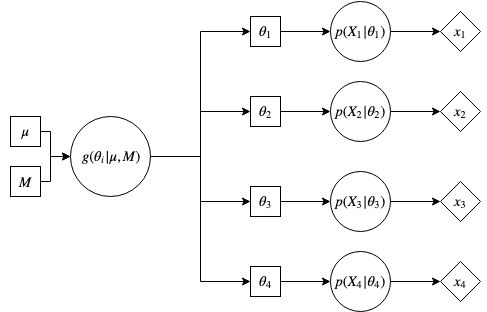
\includegraphics[height=90mm]{CT.jpg}
    \caption{A flowchart illustrating the model considered for classical test theory. Squares indicate parameters, circles indicated probability distributions, and diamonds indicate observed quantities. The hyperparameters $\mu$ and $M$ control the distribution $g(\theta_i | \mu, M)$ of true abilities $\theta_i$. For a given subject $i$, this ability serves as the mean response for each individual item in the random distribution of potential test scores $p(X_i = x_i| \theta_i)$. The observed test score $x_i$ represents one realization of this distribution. The distributions of test scores $p(X_i = x_i| \theta_i)$ are assumed to be a NEF distribution formed as a convolution of ``generating'' NEF distributions of the response for each item $Y_{ij}$, with the underlying population distribution of abilities $g(\theta_i | \mu, M)$ being conjugate to the NEF distribution.}
    \label{Fig:Flowchart}
\end{figure}

The parameters $\mu$ and $M$ of the conjugate distribution of abilities are defined by matching particular moments of the distribution.

\begin{equation}
    \begin{aligned}
        \mu = E[\theta_i]\\ 
         M = \dfrac{E[V(\theta_i)]}{Var(\theta_i)}
    \end{aligned}
    \label{Eq:Parameterization}
\end{equation}


\noindent In this parameterization, $V(\theta_i)$ is the variance function of the original $Y_{ij}$, as in Equation (\ref{Eq:QVF}). The parameter $\mu$ is the expected value of  the $\theta_i$, and it represents the population mean ability. The parameter $M$ controls, but is not equal to, the variance of $\theta_i$, how spread out the abilities are. Both are assumed, for now, to be known.

Using the law of total expectation, the unconditional expectation of the $X_i$ is

\begin{equation*}
E[X_i] = E[E[X_i | \theta_i, n_i]] = E[n_i \theta_i] = n_i \mu
\end{equation*}

\noindent and using the law of total variance, the unconditional variance of $X_i$ is

\begin{equation}
Var(X_i) = E[Var(X_i | \theta_i, n_i)] + Var(E[X_i | \theta_i, n_i]) = n_i E[ V(\theta_i)] + n_i^2 Var(\theta_i)
\label{Eq:UnconditionalVariance}
\end{equation}


\noindent In Equation (\ref{Eq:UnconditionalVariance}), the quantity $E[V(\theta_i)]$ is the average variance of the outcome of the individual test items, averaging over all possible abilities $\theta_i$. The quantity $Var(\theta_i)$ is the variance of the abilities themselves, measuring the spread of ability in the population.

%\begin{equation*}
%\theta_i | x_i, \mu, \eta \sim \dfrac{p(x_i | \theta_i)g(\theta_i | \mu, \eta)}{\int p(x_i | \theta_i)g(\theta_i | \mu, \eta) d\theta_i}
%\end{equation*}


Since $\mu$ and $M$ are assumed known, Bayes' rule can be used with conjugate prior $g(\theta_i | \mu, M)$ to calculate the posterior distribution for $\theta_i$. NEF families have closed-form posterior densities, which under conjugacy is the same density as that of the prior. For example, the result of placing a beta prior on a binomial success probability $\theta_i$ yields a beta posterior, while placing a normal prior on a normal mean $\theta_i$ yields a normal posterior. For NEF distributions with conjugate priors, the expected value of the posterior distribution for $\theta_i$ is 

\begin{equation}
 E[\theta_i | x_i, n_i, \mu, M] = \mu + (1 - B)(\bar{x_i} - \mu) = (1-B) \bar{x_i} + B \mu
\label{Eq:PosteriorMean}
\end{equation}

\noindent where $\bar{x_i}$ is the averaged score for subject $i$, obtained by dividing $x_i$ by $n_i$, and $B$ is known as the shrinkage coefficient.For NEF distributions, the form of $B$ is 

\begin{equation}
B = \change{\dfrac{E[n_i V(\theta_i)]}{Var(X_i)}} = \dfrac{n_iE[ V(\theta_i)]}{n_i E[ V(\theta_i)] + n_i^2 Var(\theta_i)} = \dfrac{E[V(\theta_i)]}{E[V(\theta_i)] + n_i Var(\theta_i)} = \dfrac{M}{M + n_i}
\label{Eq:NEFQVFB}
\end{equation} 

\noindent where $M = E[V(\theta_i)]/Var(\theta_i)$, exactly the parameterization given in Equation (\ref{Eq:Parameterization})  \citep{Morris1983}. 




%The shrinkage estimator $B$ for NEFQVF distributions is a function of two quantities: the number of test question $n_i$ and the ratio of the question-level variance for test taker $i$ to the variance of true abilities. If at a certain $n_i$ the test score tends to be very noisy around the true ability but the true abilities for all test takers tend to be clustered together, shrinkage will be large. If the test score tends to stay close to the true ability but the true abilities tend to be very spread out, shrinkage will be small. And as the number of observations $n_i$ grows bigger, the effect of the noise gets smaller, decreasing the shrinkage amount. 

%This framework assumes the values of the population parameters $M$ and $\mu$ are known. In practice, this  is unlikely to be the case. Suggestions for estimation techniques are given in Section (\ref{Sec:Estimation}), and an example is shown in Section (\ref{Sec:Example}).


\subsection{Parallel-Test Reliability}

Suppose that $X_{i,1}$ and $X_{i,2}$ are the resulting scores of subject $i$ with true ability $\theta_i$ on each of two parallel tests of length $n_i$. Each of the two tests here is assumed to be the full length of the original test. Parallel tests are defined as consisting of test items $Y_{ij,1}$ and $Y_{ij,2}$ which have the same NEF distribution with ability $\theta_i$ so that each identically and independently follows the model described in Section \ref{Subsec:NEFQVF}.

The goal is to find the correlation coefficient $\rho$ between the scores of the two tests, defined as


\begin{equation}
\rho = \dfrac{Cov(X_{i,1}, X_{i,2})}{\sqrt{Var(X_{i,1})Var(X_{i,2})}}
\label{Eq:Correlation}
\end{equation}


\noindent The numerator of Equation (\ref{Eq:Correlation}) is calculated first. The law of total covariance states that


\begin{equation}
Cov(X_{i,1}, X_{i,2}) = E[Cov(X_{i,1}, X_{i,2} | \theta_i, n_i)] + Cov(E[X_{i,1} | \theta_i, n_i], E[X_{i,2} | \theta_i, n_i]) 
\label{Eq:TotalCov}
\end{equation} 


\noindent As previously mentioned, the assumption of conditional independence for items $Y_{ij}$ given ability $\theta_i$ yields conditional independence for $X_{i,1}$ and $X_{i,2}$. The first term in Equation (\ref{Eq:TotalCov}) is then


 \begin{equation*}
E[Cov( X_{i,1},  X_{i,2} | \theta_i, n_i)] = E[0] = 0
\end{equation*}


\noindent Functionally, this means that given the same test subject $i$ the score on the first parallel test is uncorrelated with the score on the second parallel test. 

From Equation (\ref{Eq:ConditionalExpectation}), the conditional expectation is $E[ X_{i,1} | \theta_i, n_i] = E[ X_{i,2} | \theta_i, n_i] = n_i \theta_i$. The second term of Equation (\ref{Eq:TotalCov}) then becomes


\begin{equation*}
Cov(E[ X_{i,1} | \theta_i, n_i], E[ X_{i,2} | \theta_i, n_i]) = Cov\left(n_i \theta_i, n_i  \theta_i\right) = Var\left(n_i \theta_i\right) = n_i^2 Var(\theta_i)
\end{equation*}


For the denominator of Equation (\ref{Eq:Correlation}), each of $Var(X_{i,1})$ and  $Var(X_{i,2})$ can be calculated using the law of total variance as shown in Equation (\ref{Eq:UnconditionalVariance}). Since $X_{i,1}$ and $X_{i,2}$ are assumed to have the same distributional form, they will have the same variance.

\begin{equation*}
Var(X_{i,1}) = Var(X_{i,2})  = E[Var(X_{i,1} | \theta_i, n_i)] + Var(E[X_{i,1} | \theta_i, n_i]) =  n_i E[V(\theta_i)] +  n_i^2 Var(\theta_i)
\end{equation*}


\noindent where $E[V(\theta_i)]$ is the average variance of score at the level of test item. Hence, the correlation between them is

\begin{equation}
\rho = \dfrac{n_i^2 Var(\theta_i)}{n_i E[V(\theta_i)] + n_i^2 Var(\theta_i)} = 1 - \dfrac{E[V(\theta_i)]}{E[V(\theta_i)] + n_i Var(\theta_i)} = 1 - \dfrac{M}{M + n_i} = 1 - B
\label{Eq:CorrelationAsShrinkage}
\end{equation}


\noindent where $B$ is the shrinkage coefficient in Equation (\ref{Eq:NEFQVFB}) and $M = E[V(\theta_i)]/Var(\theta_i)$ as in Equation (\ref{Eq:Parameterization}). The important result, then, is that for NEF distributions, the parallel-test correlation is equal to one minus the shrinkage coefficient when a conjugate prior is used. The general formula for the parallel-test reliability of NEF distributions is 

%Since the form of the shrinkage coefficient is known for NEFQVF distributions, the test reliability can be estimated directly as a function of the parameter $M$ and the test length $n_i$.

\begin{equation}
    \rho = \dfrac{n_i}{M + n_i}
    \label{Eq:ShrinkageCorrelation}
\end{equation}

\noindent The parallel-test reliability can be calculated simply from the parameter $M$ of the underlying distribution of abilities $\theta_i$ and the test length $n_i$. In fact, if the assumptions of Section \ref{Subsec:NEFQVF} are met, the only property of the test which affects the parallel-test reliability is the test length $n_i$. \change{It should be emphasized that Equation (\ref{Eq:ShrinkageCorrelation}) occurs only when the conjugate prior distribution is used for abilities $\theta_i$.}

Equation (\ref{Eq:ShrinkageCorrelation}) has been previously derived under specific modeling assumptions. \cite{Keats1962} investigated the negative hypergeometric distribution (a form of the beta-binomial model, further described in Section \ref{Sec:Example}) and obtained Equation (\ref{Eq:ShrinkageCorrelation}) exactly -- coincidentally, with the same notation. This equation is far more general, however. It applies to the broad and flexible natural exponential family of distributions, and many commonly used formulas in classical test theory can be seen as reducing to or deriving from it. It should also be noted that the hierarchical framework of this section and derivations using laws of total expectation, variance, and covariance have also been explored for specific models, for example with the beta-binomial model in \cite{Bechger2003}, which draws connections between the classical test theory framework and item response theory. 

%This also gives a direct interpretation of the reliability as properties of the underlying distribution of abilities.  A reliability of 1 occurs if $E[V(\theta_i)]$ is zero. Given that $V(\theta_i)$ is a variance, and hence $V(\theta_i) > 0$, this implies that $V(\theta_i) = 0$ for all subjects. In terms of what this means for the test, a reliability of 1 means that every question gives an unbiased estimate of the ability with no variation. A test with a reliability of 1 would be a test in which each subject gives the same response to all test items, though the specific response may vary between test subjects. A reliability of 0 occurs when $Var(\theta_i) = 0$. In terms of what this means for the test, a reliability of 0 means that every subject has the same talent level $\theta_i$. A test with a reliability of 0 would be a test in which every subject's raw score is identical, though responses may vary within the test items that compose the raw score.



%\subsection{Discussion of Equal Difficulty Assumption}

%Perhaps the strongest assumption made is that each test question $Y_{ij}$ has mean $\theta_i$, which can be interpreted as each test question having the same ``difficulty.'' 

%For the case where both the individual responses $Y_{ij}$ and the population distribution of the abilities $\theta_i$ may be modeled using a normal density (with known variance $\sigma^2$ for the $Y_{ij}$), the independence of the mean and the variance frees the model to be equivalently written as the sum of items with unequal means and variances, or with items which consist of a constant mean and variance calculated as the average over all items. In practice, because the $Y_{ij}$ are assumed to be independent and identically distributed, the test score $X_i$ should converge to a normal density as the test length $n_i$ increases by the central limit theorem. Hence, so long as the population distribution of the abilities $\theta_i$ may be reasonably modeled using normal density, the effect of unequal question difficulties may be mitigated, though not reduced. A small simulation study displaying this phenomenon is given in Section \ref{Subsec:Simulation}.


\section{Connection to Classical Testing Theory}
\label{Sec:Connection}

%Within this framework, many of the famous results of classical testing theory are simple to derive show equivalence. The most direct is that traditional classical testing theory framework may be obtained by defining both the outcome of each test question and the distribution of abilities to be normally distributed.

%\begin{gather*}
%    Y_{ij} | \theta_i \sim N(\theta_i, \sigma^2)\\
%    X_{i} | \theta_i \sim N(n_i \theta_i, n_i\sigma^2)\\
%    \theta_i \sim N(\mu, \tau^2)
%\end{gather*}

%\noindent Then by writing $X_{i} = n_i\theta_i + \epsilon$ where $\epsilon \sim N(0,n_i \sigma^2)$, the standard form of classical test theory as a true score plus an error variance is obtained. 

 %As previously mentioned, the normal density has $V(\theta_i) = \sigma^2$, a constant which does not depend on $\theta_i$. Thus, $E[V(\theta_i)] = \sigma^2$. Using Equation (\ref{Eq:CorrelationAsShrinkage}), the parallel-test reliability is

%\begin{equation}
%    \rho = \dfrac{n_i Var(\theta_i) }{E[V(\theta_i)] + n_i %Var(\theta_i)} = \dfrac{n_i \tau^2}{\sigma^2 + n_i \tau^2} = %\dfrac{n_i}{\sigma^2/\tau^2 + n_i} = \dfrac{n_i}{M + n_i}
%    \label{Eq:NormalNormalParallelReliablity}
%\end{equation}

%\noindent In this formulation, the quantity $M$ in Equation (\ref{Eq:Parameterization}) is given by $M = \sigma^2/\tau^2$. Strictly for the purposes of calculating reliability, this is equivalent to the model

%\begin{equation}
%\begin{aligned}
%    Y_{ij} | \theta_i \sim N(\theta_i, 1)\\
%    X_{i} | \theta_i \sim N(n_i \theta_i, n_i)\\
%    \theta_i \sim N\left(\mu, \frac{1}{M} = %\frac{\tau^2}{\sigma^2}\right)
%    \end{aligned}
%    \label{Eq:NormalCTTFormulation}
%\end{equation}

%\noindent Note that $M$ is the precision, not the variance, of the distribution of talent levels. The variance is $Var(\theta_i) = \frac{1}{M}$. %Under this formulation it may be assumed, without loss of generality, that all uncertainty regarding the variance of each observation resides in the distribution of talent levels, not in the observations themselves.


The basic assumption in classical test theory that the observed score $X_i$ may be decomposed into a ``true'' component and an ``error'' component. Within the \change{generalized} framework of Section \ref{Sec:Theory}, this may be accomplished as 

%While it is possible to decompose $p(X_i | \theta_i)$ into an expectation plus a deviation from the expectation in the Bayesian framework described in Section \ref{Sec:Theory}, it is not clear that this is sensible to do except in the case where normality can be assumed. If $p(X_i | \theta_i)$ is assumed to be binomial, for example, then the ``true'' component $n_i \theta_i$ (from Equation (\ref{Eq:ConditionalExpectation})) is almost certain to be a non-integer number, in which case the subject can never achieve their ``true'' score. The distinction may be subtle, but within this framework it is more sensible to see the observed score as a random function of the ``true'' score $n_i \theta_i$.



\begin{equation}
    X_i = n_i \theta_i + \epsilon_i
    \label{Eq:TrueScorePlusError}
\end{equation}

\noindent where $n_i \theta_i$ is the ``true'' component and $\epsilon_i$ is the ``error'' component. The $\epsilon_i$ will have a distribution, but this distribution will depend on the particular NEF distribution of the $X_i$. The true score is defined as the conditional expectation of the $X_i$ given ability $\theta_i$ and test length $n_i$, as shown in Equation (\ref{Eq:ConditionalExpectation}). Then from theorem 2.1 of \cite{Novick1966}, the errors $\epsilon_i$ will have expectation 0 and the true and observed components will be uncorrelated. Since the $X_i$ are conditionally independent by assumption, the errors will also be conditionally independent, and thus uncorrelated. Thus, all general assumptions of classical test theory are met by the framework. 

%The axioms of classical test theory, as defined in \cite{Novick1966}, state that errors should have expectation 0, errors between subjects should be uncorrelated, true scores and errors within the same subject should be uncorrelated, and that there exists a linear relationship between true scores and observed scores. 


%Within the Bayesian framework, each of these may be shown to derive from assumptions.


%The expected value of $\epsilon_i$ is given by $E[\epsilon_i] = E[X_i - n_i \theta_i] = E[X_i] - n_i \theta_i = n_i \theta_i - n_i \theta_i = 0$. Hence, errors have expectation zero. Likewise, the covariance between two errors $\epsilon_{i}$ and $\epsilon_{j}$ for subjects $i$ and $j$ is given by\\


%\begin{multline*}
%    Cov(\epsilon_i, \epsilon_{j}) = E[(\epsilon_{i} - 0)(\epsilon_{j} - 0)] = E[(X_{i} - n_i\theta_i)(X_j - n_j \theta_j) ] = E[X_i X_j] - n_i \theta_i E[X_j] \\ - n_j \theta_j E[X_i] + n_i n_j \theta_i \theta_j = n_i n_j \theta_i \theta_j  - n_i n_j \theta_i \theta_j - n_i n_j \theta_i \theta_j + n_i n_j \theta_i \theta_j = 0
%\end{multline*}

%\noindent where $E[X_i X_j] = E[X_i]E[X_j]$ from the assumed independence of $X_i$ and $X_j$. Hence, the errors are uncorrelated. 

%Classical testing theory also assumes that true scores $\theta_i$ and errors $\epsilon_j$ are uncorrelated. The covariance between these two quantities is given by

%\begin{multline*}
%    Cov(\epsilon_i, n_i \theta_i) = E[(\epsilon_i - 0)(n_i \theta_i - E(n_i \theta_i)) ] = E[(X_{i} - n_i\theta_i)(n_i \theta_i - n_i \mu)] = E[n_i X_i \theta_i]  - E[n_i^2 \theta_i^2]\\ - E[n_i X_i \mu] + E[n_i^2 \mu^2]
%\end{multline*}

\cite{Novick1966} notes that while a linear regression of the observed score on the true score exists because of the decomposition in Equation (\ref{Eq:TrueScorePlusError}), a linear regression of the true score on the observed score is not true in general. It is true within the \change{generalized} classical test theory framework, however. From Equation (\ref{Eq:PosteriorMean}), the relationship between the true and observed scores is given by

\begin{equation*}
    E[n_i \theta_i | x_i, n_i, \mu, M] = B \change{n_i} \mu + (1-B) X_i = \beta_0 + \beta_1 X_i
\end{equation*}

\noindent When $X_i$ follows an exponential family distribution, this linear relationship exists if and only if $\theta_i$ follows the corresponding conjugate distribution \citep{Diaconis1979}. Hence, the use of the conjugate prior may be seen as justification for the use of a linear regression of true score on observed score. Note that the slope of the relationship is given by the reliability $\rho$. \change{Note also that when the posterior mean is taken as the estimate of true score, Equation (\ref{Eq:PosteriorMean}) and this formula are essentially Kelley's formula of \cite{Kelley1923}, which here applies to the entire natural exponential family. The application of this formula is dependent upon a linear relationship between the posterior mean and the observed score, which occurs if and only if the conjugate prior is used for abilities.}

The traditional definition of reliability as the ratio of true-score variance to observed-score variance holds. Let $\sigma^2_T = Var(n_i \theta_i) = n_i^2 Var(\theta_i)$ be the true-score variance and $\sigma^2_X$ be the observed score variance, given by Equation (\ref{Eq:UnconditionalVariance}). The ratio of true-score variance to observed-score variance is then

\begin{equation*}
    \dfrac{\sigma^2_{T}}{\sigma^2_X} = \dfrac{n_i^2 Var(\theta_i)}{n_i E[V(\theta_i)] + n_i^2 Var(\theta_i)} = \dfrac{n_i}{E[V(\theta_i)]/Var(\theta_i) + n_i} = \dfrac{n_i}{M + n_i} = \rho
\end{equation*}


Other methods of estimating reliability also reduce to simpler forms within this framework. Perhaps the most commonly used formula in classical test theory is Cronbach's alpha \citep{Cronbach1951}. Let $\sigma^2_x = Var(X_i)$ and $\sigma^2_y = Var(Y_{ij})$. The quantity $Var(X_i)$ is given by Equation (\ref{Eq:UnconditionalVariance}). Similarly, $Y_{ij}$ may be seen as a test of length $n_i = 1$ so that Equation (\ref{Eq:UnconditionalVariance}) is used to obtain $Var(Y_{ij}) = E[V(\theta_i)] + Var(\theta_i)$. Plugging these into the formula for Cronbach's alpha, it becomes

\begin{multline*}
    \alpha = \dfrac{n_i}{n_i-1} \displaystyle \left(1 - \dfrac{\sum_{i = 1}^{n_i} \sigma^2_Y}{\sigma^2_X}\right) = \dfrac{n_i}{n_i-1} \displaystyle \left(1 - \dfrac{n_i E[V(\theta_i)] + n_i Var(\theta_i)}{n_i E[V(\theta_i)] + n_i^2 Var(\theta_i)}\right) = \dfrac{n_i}{n_i-1} \displaystyle \left(1 - \dfrac{n_i M + n_i }{n_i M + n_i^2 }\right)\\
    = \dfrac{n_i}{n_i - 1}\left(\dfrac{n_iM + n_i^2 - n_i M - n_i}{n_i M + n_i^2}\right) = \dfrac{n_i}{n_i - 1}\left(\dfrac{n_i (n_i - 1)}{n_i(M + n_i)}\right) = \dfrac{n_i}{M + n_i} = \rho
\end{multline*}


\noindent Hence, Cronbach's alpha can be seen as an estimate of the parallel-test reliability in Equation (\ref{Eq:ShrinkageCorrelation}). It can also be shown that formula 21 of \cite{Kuder1937} is equivalent to Equation (\ref{Eq:ShrinkageCorrelation}) using the framework of Section \ref{Sec:Theory} and assuming a binomial distribution for test scores $X_i$, which has $V(\theta_i) = \theta_i (1 - \theta_i)$, and a beta prior distribution for $\theta_i$ \citep{Keats1962}.

The Spearman-Brown prediction formula is also easily obtained. Rearranging Equation (\ref{Eq:ShrinkageCorrelation}) gives

\begin{equation*}
    M = \left(\dfrac{1 - \rho}{\rho}\right) n_i
\end{equation*}

\noindent Suppose a reliability of $\rho$ is obtained for test length $n_i$, but the test length $\tilde{n}_i$ which yields reliability $\tilde{\rho}$ is desired. Equating $M$  for each formula gives

\begin{equation*}
     \left(\dfrac{1 - \rho}{\rho}\right) n_i = \left(\dfrac{1 - \tilde{\rho}}{\tilde{\rho}}\right) \tilde{n}_i
\end{equation*}

\noindent and rearranging terms gives

\begin{equation*}
    \dfrac{\tilde{n_i}}{n_i} = \dfrac{\tilde{\rho}(1 - \rho)}{\rho (1 - \tilde{\rho})}
\end{equation*}

Lastly, though not a focus of this paper, the framework of Section \ref{Subsec:NEFQVF} is easily expanded to deal with violated assumptions. A very strong assumption made is that the response $Y_{ij}$ to each item has mean $\theta_i$, assuming in essence that each item is the same difficulty. In practice, this is commonly not the case. This can be addressed by modeling the transformed $\theta_i$ values as a function of a subject effect and an item effect. For example, suppose that the $Y_{ij}$ are Bernoulli random variables with $P(Y_{ij} = 1) = \theta_{ij}$. Then modeling

\begin{equation*}
    \log \left(\dfrac{\theta_{ij}}{1-\theta_{ij}}\right) = \alpha_i + \beta_j
\end{equation*}

\noindent where $\alpha_i$ is a subject effect and $\beta_i$ is an item effect yields a basic item response theory (IRT) model \citep{Gelman2007}. \change{This derivation, using convolutions of independent exponential family distributions as in Section \ref{Subsec:NEFQVF}, is similar to work found in \cite{Rasch1960}. The use of non-conjugate distributions for $\theta_i$ induces a non-linear regression of ability (estimated as the posterior mean) on observed score. Conversely, the linear regression induced by the conjugate distribution might be seen as mirroring an IRT procedure with no item parameters and no guessing, where trait or ability is simply randomly distributed within the population.}

%The use of the logit function in a procedure like IRT might be seen as an attempt to maintain a linear regression while modeling the ability as a function of covariates rather than a population mean, or conversely, the framework here might be seen as a no-covariate procedure, where trait/ability is simply randomly distributed within the population.

\section{Inference}
\label{Sec:Estimation}

The formulation of reliability in Section \ref{Sec:Theory} and derivations of classical test theory properties in Section \ref{Sec:Connection} have thus far assumed that the parameters $\mu$ and $M$ of the underlying distribution of abilities $\theta_i$ are known. In rare cases, there may exist strong prior information which can be used to determine appropriate values to plug in. In most cases, these parameters must be estimated. 

%This formulation of classical testing theory in a Bayesian framework opens new avenues for estimation. By formulating the problem in terms of the uncertainty can be estimated by traditional techniques and then propagated through to estimates of reliability. 


\subsection{Estimation Methods for $\mu$ and $M$}
\label{Subsec:EstimationTechniques}

%The common classical test theory statistics such as Cronbach's alpha rely upon moment-based estimates, typically derived from correlations among test items. If

Maximum likelihood estimation is natural choice for estimation. The act of estimating the parameters of the underlying conjugate distribution of abilities \change{by marginal maximum likelihood} and then using them as plug-in estimates to obtain quantities of interest from the posterior distribution makes this an empirical Bayes approach.

The marginal distribution of observed score $X_i$ unconditional on the ability $\theta_i$ is obtained by integrating the product of the score distribution and the conjugate prior distribution over $\theta_i$.

\begin{equation}
    f(x_i | \mu, M, n_i) = \displaystyle \int_{\theta_i} p(x_i | \theta_i, n_i) g(\theta_i | \mu, M) d\theta_i \label{Eq:MarginalDensity}
\end{equation}

\noindent In the case of a normal distribution for both $X_i$ and $\theta_i$, this marginal density is also normally distributed, simplifying calculations. Other scenarios are more complicated. A complete description of the relationships between the six NEF distributions with quadratic variance function, their conjugate priors, and their marginal distributions can be found in \cite{Morris2009}, and a thorough description of their application in this framework can be found in the Appendix. The marginal density in Equation (\ref{Eq:MarginalDensity}) gives a direct formula for the observed test scores in terms of the desired parameters, and the maximum likelihood estimates $\hat{\mu}$ and $\hat{M}$ are obtained by maximizing the log-likelihood.

\begin{equation*}
(\hat{\mu}, \hat{M}) = \displaystyle \arg \max_{(\mu, M)} \sum_{i = 1}^K \log[f(x_i | \mu, M, n_i)]
\end{equation*}

\noindent When neither the distribution of test scores or abilities are normally distributed, this maximization is typically performed with an iterative optimization routine using a computer. An example using the binomial model with a beta prior is given in Section \ref{Sec:Example}. 

The advantage of maximum likelihood using an iterative optimization routine is that it presents a direct method of obtaining variance estimates of the parameters as

\begin{equation}
    Var(\hat{M}) \approx -J_n^{-1}(\hat{M})
    \label{Eq:MVariance}
\end{equation}

\noindent where $\hat{M}$ is the maximum likelihood estimate and $-J_n^{-1}(\hat{M})$ is the observed Fisher information at $\hat{M}$ \citep{CasellaBerger}. This is obtained by calculating the matrix of second partial derivatives of the log-likelihood, called the Hessian matrix, and inverting it at the maximum likelihood estimates $\hat{\mu}$ and $\hat{M}$. As many iterative optimization routines rely on this matrix for determining the direction of the step at each iteration, it may be available. If unavailable, it can calculated numerically.

%Maximum likelihood estimates $\hat{\mu}$ and $\hat{M}$ may then be inserted directly into Equation (\ref{Eq:ShrinkageCorrelation}) to estimate the test reliability. This method is known as parametric empirical Bayes, and a full example is given in Section \ref{Sec:Example}.

 Another option is to place a hyperprior or hyperpriors on $\mu$ and $M$ and perform a full hierarchical Bayesian analysis, which will almost certainly involve Markov chain Monte Carlo sampling. This method is of particular interest where moderately informative prior information may exist about the values of $\mu$ and $M$. Prior sensitivity of the analysis will likely be an issue, especially for small sample sizes. A thorough description of MCMC techniques in psychometrics is given in \cite{Levy2016}.



\subsection{Empirical Bayesian Point and Interval Estimates for Reliability and Test Length}
\label{Subsec:IntervalFormulas}

Given maximum likelihood estimates $\hat{\mu}$ and $\hat{M}$, Equation (\ref{Eq:ShrinkageCorrelation}) gives the estimated parallel-test reliability as

\begin{equation}
    \hat{\rho} = \dfrac{n_i}{n_i + \hat{M}}
    \label{Eq:EstimatedReliability}
\end{equation}

\noindent By the invariance of the maximum likelihood estimator, $\hat{\rho}$ is the maximum likelihood estimate of the parallel-test reliability. Note that in Equation (\ref{Eq:EstimatedReliability}) the test length $n_i$ is both constant and indexed by subject $i$. This has two consequences: first, that the test reliability may vary between subjects if the test length $n_i$ varies as well. Second, the reliability may be calculated for any test length, not just the test length $n_i$ used to obtain $\hat{M}$. Supposing one is considering extending the test to new length $\tilde{n_i}$, the new test length may simply be inserted into Equation (\ref{Eq:EstimatedReliability})  in order to obtain the maximum likelihood estimate of the parallel-test reliability for that test length.

Assuming the variance for $\hat{M}$ is available, likely from the observed Fisher information obtained by taking the appropriate element of the negative inverted Hessian matrix as in Equation (\ref{Eq:MVariance}) , it can be converted to a variance for the estimated reliability $\hat{\rho}$ by the delta method.

\begin{equation*}
Var(\hat{\rho}) \approx \left[\dfrac{d}{d \hat{M}} \left(\dfrac{n_i}{n_i + \hat{M}}\right) \right]^2 Var(\hat{M}) = \left(\dfrac{n_i^2}{(n_i + \hat{M})^4}\right) Var(\hat{M})
\end{equation*}

\noindent A $(1 - \alpha) \times 100\%$ interval for $\hat{\rho}$ is then given by

\begin{equation}
    \left(\dfrac{n_i}{n_i + \hat{M}}\right) \pm z^* \left(\dfrac{n_i}{(n_i + \hat{M})^2}\right) \sqrt{Var(\hat{M})}
    \label{Eq:RhoInterval}
\end{equation}

\noindent where $z^*$ is the $(1 - \frac{\alpha}{2})$ quantile of the standard normal density.

An interval estimate of the sample size required for a desired reliability is also easily obtained. Given the desired reliability $\rho$, the estimated test length $n_i$ which will provide the reliability is


\begin{equation}
\hat{n_i} = \left(\dfrac{\rho}{1-\rho}\right)\hat{M}
\label{Eq:ProphecyPoint}
\end{equation}

\noindent The variance of the estimated test length for reliability $\rho$ is


\begin{equation*}
Var(\hat{n_i}) = Var\left( \left(\dfrac{\rho}{1-\rho}\right)\hat{M}\right) = \left(\dfrac{\rho}{1-\rho}\right)^2 Var(\hat{M})
\end{equation*}


\noindent and so a $(1-\alpha)\times 100\%$ interval for $\hat{n_i}$ is given as


\begin{equation}
\left(\dfrac{p}{1-p}\right)\hat{M} \pm z^* \left(\dfrac{p}{1-p}\right) \sqrt{Var(\hat{M})}
\label{Eq:ProphecyInterval}
\end{equation}

\noindent where $z^*$ is once again the $(1 - \frac{\alpha}{2})$ quantile of the standard normal density.

Lastly, suppose the goal is inference for the estimated reliability if the test length is increased to $\tilde{n_i}$. A point estimate is given by

\begin{equation}
    \hat{\rho} = \dfrac{\tilde{n_i}}{\tilde{n_i} + \hat{M}}
    \label{Eq:ReliabilityPoint}
\end{equation}

\noindent with the delta method yielding a corresponding $(1 - \alpha) \times 100\%$ interval given by

\begin{equation}
    \dfrac{\tilde{n_i}}{\tilde{n_i} + \hat{M}} \pm z^* \left(\dfrac{\tilde{n_i}}{(\tilde{n_i} + \hat{M})^2}\right) \sqrt{Var(\hat{M})}
    \label{Eq:ReliabilityInterval}
\end{equation}

Each of the standard errors for the interval estimates is derived from the Fisher information, which depends on asymptotic normality of the maximum likelihood estimator for accuracy. This asymptotic normality in turn depends on both the test lengths $n_i$ and the number of subjects being sufficiently large. When either of these is small, the standard error may be incorrect. 

The delta method is, of course, not the only way to obtain variance estimates of the reliability and derived quantities. If a hierarchical Bayesian analysis is performed with MCMC, draws from the posterior distribution for $M$ may be inserted directly into Equation (\ref{Eq:EstimatedReliability}) in order to obtain a posterior distribution for $\rho$ or into Equation (\ref{Eq:ProphecyPoint}) to obtain a posterior distribution for $\hat{n}_i$. The bootstrap is another option. Both of these will remain sensitive to small sample sizes, a problem for which there is unfortunately no magical cure.

\section{Example and Simulation Study}
\label{Sec:Example}

The presentation thus far has been purely theoretical. An example may show how the theory is applied in practice. Suppose that the results of a multiple-choice test are available. This example uses the multiple-choice data included with the R package `CTT' by \cite{Willse2018}. The data consists of the per-item responses on a $n_i = 20$ item multiple choice test conducted on $K = 100$ subjects. Each response is treated as dichotomous, with 0 for an incorrect response and 1 for a correct response. Each subject is assumed to have true ability $\theta_i$, which is unique to each subject and remains constant over all items. The observed scores and number of subjects with the associated scores are shown in Table \ref{Table:ExampleData}.


\begin{table}
    \centering
    \begin{tabular}{| c | c ||  c | c |} \hline
    Score & Freq. & Score & Freq. \\ \hline
    1 & 1 & 11 & 1 \\
    2 & 1 & 12 & 10 \\
    3 & 2 & 13 & 8 \\
    4 & 7 & 14 & 2 \\
    5 & 13 & 15 & 6 \\
    6 & 6 & 16 & 1 \\
    7 & 14 & 17 & 4 \\
    8 & 5 & 18 & 3 \\
    9 & 7 & 19 & 2 \\
    10 & 6 & 20 & 1 \\ \hline
    \end{tabular}
\caption{Observed score and corresponding frequency from the example data provided with the R package `CTT' package \cite{Willse2018}. The responses are available in the package on a per-item basis, but only the total scores are shown here.}
\label{Table:ExampleData}
\end{table}

\subsection{Beta-Binomial Formulation}
\label{Subsec:BetaBinomial}

Under this formulation, the observed score $x_i$ for subject $i$ should be modeled as following a binomial random variable with success probability $\theta_i$. The probability mass function is

\begin{equation*}
    p(x_i | \theta_i, n_i) = {n_i \choose x_i} \theta^{x_i} (1-\theta_i)^{x_i} 
\end{equation*}

The distribution of abilities $\theta_i$ is assumed to follow the conjugate prior for the binomial mass function, commonly known as the beta distribution. Traditionally, the parameters of a beta distribution are written as $\alpha$ and $\beta$. For this paper, the parameterization given in Equation (\ref{Eq:Parameterization}) is used. In terms of $\alpha$ and $\beta$, this is

\begin{align*}
    \mu = \dfrac{\alpha}{\alpha + \beta}\\
    M = \alpha + \beta
\end{align*}

\noindent This yields $\alpha = \mu M$ and $\beta = (1 - \mu) M$. The density of the prior is then 

\begin{equation*}
    g(\theta_i | \mu, M) = \dfrac{\theta_i^{\mu M -1} (1 - \theta_i)^{(1-\mu)M - 1}}{\beta(\mu M, (1 - \mu)M)}
\end{equation*}

Integrating out the ability $\theta_i$, the unconditional density of the observed test score $x_i$ in terms of the population parameters is given by

\begin{equation}
    f(x_i | \mu, M) = \displaystyle \int_{\theta_i} p(x_i | \theta_i) g(\theta_i | \mu, M) d\theta_i =  {n_i \choose x_i} \dfrac{\beta(x_i + \mu M, n_i - x_i + (1 - \mu)M}{\beta(\mu M, (1 - \mu)M)}
    \label{Eq:BetaBinomialDensity}
\end{equation}

\noindent The distribution in Equation (\ref{Eq:BetaBinomialDensity}) is known as the beta-binomial distribution and represents the potential distribution of the test score $x_i$ in $n_i$ observations if the subject $i$ is unknown. More importantly, this distribution will serve as the basis for estimation and inference. Given a set of test scores for $K$ subjects, the log-likelihood for parameters $\mu$ and $M$ is given by

\begin{equation}
    \ell(\mu, M) = \left(\displaystyle \sum_{i = 1}^K \log[\beta(x_i + \mu M, n_i - x_i + (1 - \mu)M)]\right) - K\log[\beta(\mu M, (1 - \mu)M)]
    \label{Eq:BBLogLikelihood}
\end{equation}

\noindent Maximizing Equation (\ref{Eq:BBLogLikelihood}) using observed scores $x_i$ and test lengths $n_i$ yields the maximum likelihood estimates $\hat{\mu}$ and $\hat{M}$. As Equation (\ref{Eq:BBLogLikelihood}) is not analytically tractable, this is typically done with an iterative numerical solver. Similar derivations of the properties of NEF models other than the beta-binomial are given in the Appendix.

%The primary advantage of . Many iterative numerical solvers make use of the Hessian matrix $H$, the matrix of partial second derivatives of the log-likelihood function given in Equation (\ref{Eq:BBLogLikelihood}), 

%\noindent where $-H^{-1}_{MM}$ is the element of the negative inverse Hessian matrix corresponding to two sequential partial derivatives of the log-likelihood in Equation (\ref{Eq:BBLogLikelihood}) both taken with respect to $M$. These maximum likelihood estimates are guaranteed to be asymptotically unbiased, but can be biased in finite sample sizes.


%\cite{CasellaBerger}

\subsection{Analysis}
\label{Subsec:RealExample}

For the example data of the `CTT' package, the maximum likelihood estimates obtained by maximizing Equation (\ref{Eq:BBLogLikelihood}) are $\hat{\mu} = 0.480$ and $\hat{M} = 5.334$.  The optimization was performed using the default ``optim'' command in the R programming language. This routine can be specified to return the Hessian matrix. The estimated variance of $\hat{M}$, given by the negative inverse of the Hessian matrix as in Equation (\ref{Eq:MVariance}), is $Var(\hat{M}) \approx 0.874$. The estimated parallel-test reliability is then

\begin{equation*}
    \hat{\rho} = \dfrac{20}{20 + 5.334} \approx 0.789
\end{equation*}

\noindent with corresponding 95\% interval estimate
\begin{equation*}
    0.789 \pm 1.96 \left(\dfrac{20}{(20+5.334)^2}\right) \sqrt{0.874} = (0.732, 0.847)
\end{equation*}

A traditional method of calculating the reliability of dichotomously-scored test data  is formula 20 of \cite{Kuder1937}. The KR-20 estimate of reliability for this data set is $0.815$ with a 95\% interval of $(0.758, 0.864)$ using the method of \cite{Feldt1965} and \cite{Feldt1987}. Similarly, the KR-21 estimate of reliability for this data set is $0.796$ with 95\% interval $(0.732,0.850)$. Unsurprisingly, the empirical Bayesian estimates of reliability and the KR-21 estimates of reliability are close in value, having made the same assumption of equality of test item difficulty. 

Suppose that a reliability of $\rho = 0.9$ is desired for the test as a whole. Then following Equation (\ref{Eq:ProphecyPoint}), the estimated test length $\hat{n}_i$ is 

\begin{equation*}
    \hat{n}_i = \left(\dfrac{0.9}{1-0.9}\right) 5.334 \approx 48
\end{equation*}

\noindent with corresponding 95\% interval, following Equation (\ref{Eq:ProphecyInterval}), equal to

\begin{equation*}
    48 \pm 1.96 \left(\dfrac{0.9}{1-0.9}\right) \sqrt{0.874} = (31.50, 64.50)
\end{equation*}

Likewise, suppose that the test length is to be increased to $\tilde{n_i} = 30$ items. The estimated reliability from Equation (\ref{Eq:ReliabilityPoint}) is then

\begin{equation*}
    \hat{\rho} = \dfrac{30}{30 + 5.334} \approx 0.849
\end{equation*}

\noindent with corresponding 95\% interval, from Equation (\ref{Eq:ReliabilityInterval}), equal to

\begin{equation*}
    0.849 \pm 1.96 \left(\dfrac{30}{(30+5.334)^2}\right) \sqrt{0.874} = (0.805, 0.893)
\end{equation*}

These can be repeated to give interval estimates for any desired reliability $\rho$ or new test length $\tilde{n_i}$. A plot of estimated reliability as a function of the test length with 95\% bounds and a plot of the estimated test length as a function of the reliability with 95\% bounds are shown in Figure \ref{Fig:ErrorPlots}.


\begin{figure}
    \centering
    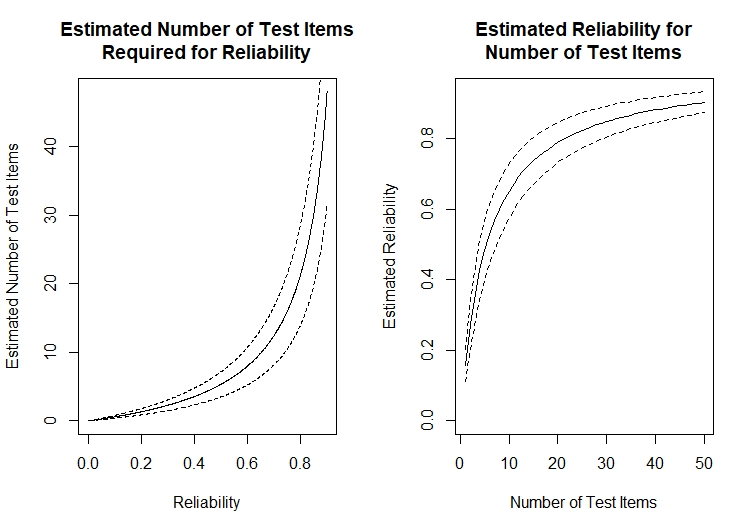
\includegraphics[height = 110mm]{Plots.jpeg}
    \caption{On the left, a plot showing the estimated test length $\hat{n}_i$ required to obtain a test reliability of $\rho$, with 95\% error bounds. The estimate and error bounds are calculated using Equations (\ref{Eq:ProphecyPoint}) and (\ref{Eq:ProphecyInterval}). On the right, a plot showing the estimated reliability $\hat{\rho}$ for a given test length $\tilde{n_i}$, with 95\% error bounds. The estimate and error bounds are calculated using Equations (\ref{Eq:ReliabilityPoint}) and (\ref{Eq:ReliabilityInterval}). Both plots are calculated for the example data included with the `CTT' package of \cite{Willse2018}, given in Table \ref{Table:ExampleData}.}
    \label{Fig:ErrorPlots}
\end{figure}


\subsection{Simulation Study}
\label{Subsec:Simulation}

The example of Section \ref{Subsec:RealExample} is useful for showing rough equivalence of the empirical Bayesian and classical estimators of reliability for a single data set, but it is unable to show properties of interval estimators. For this, a simulation study is necessary.

The beta-binomial model of Section \ref{Subsec:BetaBinomial} can be used to simulate sets of observed test scores. For this simulation study, three sets of parameters $\mu$ and $M$ were chosen. The first set, with $\mu = 0.75$ and $M = 4$, yields a distribution of abilities which is unimodal with mean 0.75, but skewed to the left rather than symmetric. The second set, with $\mu = 0.5$ and $M = 1$, is the classic Jeffrey's prior for a binomial success probability. This distribution of abilities is U-shaped with a mean of 0.5, symmetric, but with no mode. The last set, with $\mu = 0.5$ and $M = 20$, is unimodal, symmetric, and nearly bell-shaped, with only a slight divergence at the tails. For each set of parameters, five sets of test length $n_i$ and number of subjects $K$ were used. These were $n_i = 10$ and $K = 10$, which is small in both and so should pose difficulties in estimation, and each combination of $n_i = 30$ or $100$ and $K = 30$ or $100$, presenting a moderate or large sample size in each category.

The target of estimation is the true parallel-test reliability in Equation (\ref{Eq:ShrinkageCorrelation}). The accuracy of the estimator is judged both pointwise and with 95\% intervals. For pointwise accuracy, the root mean squared error is used.

\begin{equation*}
    RMSE = \sqrt{\dfrac{1}{N_{sims}} \displaystyle \sum_{s = 1}^{N_{sims}} (\rho - \hat{\rho}_{s})^2}
\end{equation*}

\noindent For interval accuracy, the empirical coverage is used. All intervals are calculated as 95\% intervals.

A total of $N_{sims} = 100000$ simulated data sets were created for each set of parameters. For each simulated data set, both a point and 95\% interval estimate of reliability are calculated using the empirical Bayesian estimators of Section \ref{Sec:Estimation} and the classical formula 20 of \cite{Kuder1937} with corresponding interval given by \cite{Feldt1965} and \cite{Feldt1987}, the default interval implemented in SPSS. The results of the simulation study are shown below in Table \ref{Table:SimulationStudy}. 

\begin{table}
    \centering
    \begin{tabular}{| c | c | c | c | c || c | c || c | c |} \hline
     $\mu$ & $M$ & $n_i$ & $K$ & $\rho$ & EB RMSE & Coverage & KR20 RMSE & Coverage\\ \hline
        0.75 & 4 & 10 & 10 & 0.714 & 0.244 & 0.914 & 0.233 & 0.885\\ % Redone*
        0.75 & 4 & 30 & 30 & 0.882 & 0.040 & 0.956 & 0.038 & 0.917\\ % Redone
        0.75 & 4 & 30 & 100 & 0.882 & 0.019 & 0.953 & 0.019 & 0.925\\ % Redone
        0.75 & 4 & 100 & 30 & 0.962 & 0.013 & 0.957 & 0.012 & 0.919 \\ % Redone
        0.75 & 4 & 100 & 100 & 0.962 & 0.006 & 0.952 & 0.006 & 0.928\\ % Redone
        0.50 & 1 & 10 & 10 & 0.909 & 0.078 & 0.941 & 0.062 & 0.800\\ % Redone
        0.50 & 1 & 30 & 30 & 0.968 & 0.009 & 0.953 & 0.009 & 0.906\\ % Redone
        0.50 & 1 & 30 & 100 & 0.968 & 0.005 & 0.950 & 0.005 & 0.934\\ % Redone  
        0.50 & 1 & 100 & 30 & 0.990 & 0.003 & 0.953 & 0.003 & 0.922\\ % Redone
        0.50 & 1 & 100 & 100 & 0.990 & 0.001 & 0.952 & 0.001 & 0.938\\ % Redone*
        0.50 & 20 & 10 & 10 & 0.333 & 0.245 & 0.620 & 0.515 & 0.926\\ % Redone
        0.50 & 20 & 30 & 30 & 0.600 & 0.132 & 0.957 & 0.119 & 0.944\\ % Redone
        0.50 & 20 & 30 & 100 & 0.600 & 0.061 & 0.953 & 0.059 & 0.952\\ % Redone 
        0.50 & 20 & 100 & 30 & 0.833 & 0.055 & 0.957 & 0.049 & 0.946\\ % Redone
        0.50 & 20 & 100 & 100 & 0.833 & 0.025 & 0.953 & 0.024 & 0.953\\ \hline % Redone
    \end{tabular}
\caption{Results of simulation experiment, simulating from the beta-binomial model described in Section \ref{Subsec:BetaBinomial}. The target of estimation is the true parallel test reliability given by $n_i/(n_i + M)$ in Equation (\ref{Eq:ShrinkageCorrelation}). The first four columns give the true population parameters $\mu$ and $M$ used to simulate the data. The parameter $n_i$ is the number of test items and the parameter $K$ is number of subjects. A total of $N_{sims} = 100000$ data sets were simulated for each set of parameters. For each set of parameters, the test reliability and nominal 95\% interval coverage were calculated using the empirical Bayes approach of Section \ref{Subsec:EstimationTechniques} and implemented in Section \ref{Subsec:RealExample}. This is compared to the estimated reliability using \cite{Kuder1937} formula 20 and nominal 95\% interval using the method from \cite{Feldt1965} and \cite{Feldt1987}. }
\label{Table:SimulationStudy}
\end{table}
\newpage

In general, the empirical Bayesian estimator gives a slight increase in RMSE as compared to Kuder and Richardson's formula 20, but with the advantage of providing closer to nominal coverage. The scenario was reversed, however, with the set of parameters $\mu = 0.50, M = 20$, and $n_i = K = 10$, in which the empirical Bayesian method struggled to accurately estimate the underlying variance of abilities when observed scores tended to be clustered together due to both the small sample size and the unimodal and symmetric shape of the distribution of abilities, while the KR-20 method produced more accurate interval estimates. Taken as a whole, it is clear that the empirical Bayesian estimates of reliability are close to traditional formulas for reliability in terms of both point and interval estimation.

%Though not shown, Kuder and Richardson's formula 21 point estimate and corresponding interval estimate were also calculated for each data set. These tended to show slightly better RMSE than the empirical Bayesian estimator, but slightly worse coverage than the KR-21 intervals, essentially acting as a ``compromise'' estimator. 

% $\hat{M}$ from the empirical Bayesian estimator is biased, and Kuder and Richardson's formula 20 exhibits no such bias. 

%The most likely explanation for the decreased RMSE is that maximum likelihood estimators are only guaranteed to be unbiased asymptotically, while moment-based formulas such as \cite{Kuder1937} formula 20 exhibit no such bias. 

%Though not shown, \cite{Kuder1937} formula 21 was also calculated for each data set. The RMSE for the KR21 estimate is slightly higher than KR20, but below the EB RMSE, while the interval coverage is slightly lower than the EB coverage, but higher than the KR20 coverage. It can be seen as representing an intermediate estimator between the empirical Bayesian reliability estimate and the KR-21.


\section{Discussion and Conclusion}

%The framework presented in this paper is not intended to replace classical test theory, but rather to expand it.

It has been shown that, when unidimensionality and equal item difficulty are assumed, many of the results of classical test emerge directly from the theory of natural exponential families and \change{Bayesian theory of} their conjugate priors. When this broader theory is taken into account, it allows for a rich inferential framework which is amenable to \change{common techniques for hierarchical models}. Estimates from this framework are competitive, in terms of common measures such as root mean squared error and coverage of intervals, with traditional classical test theory formulas.

The framework can and should be extended, as assumptions of classical test theory are often violated in practice. The \change{generalized} framework presents direct ways in which these violated assumptions may be incorporated into a model.  For example, it has already been noted that modeling abilities as a function of both subject and item leads directly to an item response model, but there is no reason to limit this to dichotomous data. The NEF assumption allows the framework to extend naturally into generalized linear model theory. Poisson count data, geometric counts of the number of trials until success, or negative binomial counts of the number of successes until a given number of failures may all be modeled in this manner as well. The relatively modest framework here may be embedded into more complicated hierarchical models in order to adapt to peculiar aspects of the test data at hand, such as changing abilities over time or multiple subgroups within the population. \change{It may also be possible to expand the framework to multi-parameter test items through the use of multivariate analogues of natural exponential families, for example by modeling polytomous responses using the Dirichlet-multinomial similarly to modeling dichotomous responses using the beta-binomial}. The term framework is appropriate - it is a small piece to be built upon, in order to create a larger whole model which may address the problem at hand.


%The Bayesian method for calculating estimates for the reliability is can easily handle missing or omitted information as well. Note that none of the formulas given in this paper require that the test length $n_i$ be the same for all subjects $i$. Because of this, omitted questions may simply be removed and $n_i$ adjusted accordingly. In fact, the method does not even require that the subjects take the same test so long as the test scores $X_i$ follow the assumptions given in Section \ref{Sec:Theory}. 


%If there is perhaps an application in which this framework can prove useful, it is the estimation of standard errors associated with psychometric quantities. Standard errors for quantities such as Cronbach's alpha are are difficult to derive and sensitive to assumptions of normality. By modeling these quantities as direct functions of model parameters, the uncertainty in the model parameters can easily be propagated through to the quantity of interest, though this may require computing techniques such as Markov chain Monte Carlo. %Indeed, as Section \ref{Subsec:Simulation} shows, interval estimates derived from posterior distributions may hold coverage well under a variety of true ability distributions.


% BIBLIOGRAPHY 

%% HERE WE DECLARE THE BIBLIOGRAPHYSTYLE TO USE AND THE BIBLIOGRAPHY DATABASE
%\bibliographystyle{apacite}

\clearpage
\bibliographystyle{apacite}
%\bibliographystyle{plainnat}
%\bibliographystyle{apalike}
\begin{thebibliography}{28}
\providecommand{\natexlab}[1]{#1}
\providecommand{\url}[1]{\texttt{#1}}
\expandafter\ifx\csname urlstyle\endcsname\relax
  \providecommand{\doi}[1]{doi: #1}\else
  \providecommand{\doi}{doi: \begingroup \urlstyle{rm}\Url}\fi

\bibitem[Bechger, Maris, Verstralen, and
  B\'eguin(2003)]{Bechger2003}%Bechger et~al.
Timo~M. Bechger, Gunter Maris, Huub H. F.~M. Verstralen, and Anton~A. B\'eguin.
\newblock Using classical test theory in combination with item response theory.
\newblock \emph{Applied Psychological Measurement}, 27\penalty0 (5):\penalty0
  319 -- 334, September 2003.

\bibitem[Casella and Berger(2002)]{CasellaBerger}
G~Casella and R~Berger.
\newblock \emph{Statistical Inference, Second Edition}.
\newblock Duxbury Press, 2002.

\bibitem[Cronbach(1951)]{Cronbach1951}
Lee~J. Cronbach.
\newblock Coefficient alpha and the internal structure of tests.
\newblock \emph{Psychometrika}, 16\penalty0 (3):\penalty0 297 -- 334, September
  1951.

\bibitem[Diaconis and Ylvisaker(1979)]{Diaconis1979}
Persi Diaconis and Donald Ylvisaker.
\newblock Conjugate priors for exponential families.
\newblock \emph{The Annals of Statistics}, 7\penalty0 (2):\penalty0 269 -- 281,
  1979.

\bibitem[Feldt(1965)]{Feldt1965}
Leonard~S. Feldt.
\newblock The approximate sampling distribution of kuder-richardson reliability
  coefficient twenty.
\newblock \emph{Psychometrika}, 30\penalty0 (3):\penalty0 357 -- 370, September
  1965.

\bibitem[Feldt, Woodruff, and Salih(1987)]{Feldt1987}%Feldt et~al.
Leonard~S. Feldt, David~J. Woodruff, and Fathi~A. Salih.
\newblock Statistical inference for coefficient alpha.
\newblock \emph{Applied Psychological Measurement}, 11\penalty0 (1):\penalty0
  93 -- 103, March 1987.

\bibitem[Gelman and Hill(2007)]{Gelman2007}
Andrew Gelman and Jennifer Hill.
\newblock \emph{Data analysis using regression and multilevel/hierarchical
  model}.
\newblock Cambridge University Press, 2007.

\bibitem[Keats and Lord(1962)]{Keats1962}
J.~A. Keats and Frederic~M. Lord.
\newblock A theoretical distribution for mental test scores.
\newblock \emph{Psychometrika}, 27\penalty0 (1):\penalty0 59 -- 72, March 1962.

\bibitem[Kelley(1923)]{Kelley1923}
T.L. Kelley.
\newblock \emph{Statistical method}.
\newblock New York: Macmillan, 1923.

\bibitem[Kuder and Richardson(1937)]{Kuder1937}
G.~F. Kuder and M.~W. Richardson.
\newblock The theory of the estimation of test reliability.
\newblock \emph{Psychometrika}, 2\penalty0 (3):\penalty0 151 -- 160, 1937.

\bibitem[Levy and Mislevy(2016)]{Levy2016}
Roy Levy and Robert~J. Mislevy.
\newblock \emph{Bayesian psychometric modeling}.
\newblock Chapman \& Hall/CRC, 2016.

\bibitem[Li and Woodruff(2002)]{Li2002}
Jun~Corser Li and David~J. Woodruff.
\newblock Bayesian statistical inference for coefficient alpha.
\newblock Technical report, ACT Research Report Series, 2002.

\bibitem[Lindley(1969{\natexlab{a}})]{Lindley1969}
Dennis~V. Lindley.
\newblock A bayesian solution for some educational prediction problems.
\newblock Technical report, Educational Testing Service, Princeton, New Jersey,
  July 1969{\natexlab{a}}.

\bibitem[Lindley(1969{\natexlab{b}})]{Lindley1969b}
Dennis~V. Lindley.
\newblock A bayesian estimate of true score that incorporates prior
  information.
\newblock Technical report, Educational Testing Service, 1969{\natexlab{b}}.

\bibitem[Lord(1965)]{Lord1965}
Frederic~M. Lord.
\newblock A strong true-score theory, with applications.
\newblock \emph{Psychometrika}, 30\penalty0 (3):\penalty0 239 -- 270, September
  1965.

\bibitem[Lord(1969)]{Lord1969}
Frederic~M. Lord.
\newblock Estimating true-score distributions in psychological testing (an
  empirical bayes estimation problem).
\newblock \emph{Psychometrika}, 34\penalty0 (3):\penalty0 259 -- 299, September
  1969.

\bibitem[Lord, Novick, and Birnbaum(1968)]{Lord1968}%Lord et~al.
Frederic~M. Lord, Melvin~R. Novick, and Allen Birnbaum.
\newblock \emph{Statistical theories of mental test scores}.
\newblock Addison-Wesley, Oxford, England, 1968.

\bibitem[Morris(1982)]{Morris1982}
Carl~N. Morris.
\newblock Natural exponential families with quadratic variance functions.
\newblock \emph{The Annals of Statistics}, 10\penalty0 (1):\penalty0 65 -- 80,
  1982.

\bibitem[Morris(1983)]{Morris1983}
Carl~N. Morris.
\newblock Natural exponential families with quadratic variance functions:
  Statistical theory.
\newblock \emph{The Annals of Statistics}, 11\penalty0 (2):\penalty0 515 --
  529, 1983.

\bibitem[Morris and Lock(2009)]{Morris2009}
Carl~N. Morris and Kari~F. Lock.
\newblock Unifying the named natural exponential families and their relatives.
\newblock \emph{The American Statistician}, 63\penalty0 (3):\penalty0 247 --
  253, August 2009.

\bibitem[Najafabadi and Najafabadi(2016)]{Najafabadi2016}
Amir T.~Payandeh Najafabadi and Maryam~Omidi Najafabadi.
\newblock On the bayesian estimation for cronbach's alpha.
\newblock \emph{Journal of Applied Statistics}, 43\penalty0 (13):\penalty0 2416
  -- 2441, 2016.

\bibitem[Novick(1966)]{Novick1966}
Melvin~R. Novick.
\newblock The axioms and principal results of classical test theory.
\newblock \emph{Journal of Mathematical Psychology}, 3\penalty0 (1):\penalty0 1
  -- 18, 1966.

\bibitem[Novick(1969{\natexlab{a}})]{Novick1969}
Melvin~R. Novick.
\newblock Multiparameter bayesian indifference procedures.
\newblock \emph{Journal of the Royal Statistical Socity. Series B
  (Methodological)}, 31\penalty0 (1):\penalty0 29--64, 1969{\natexlab{a}}.

\bibitem[Novick(1969{\natexlab{b}})]{Novick1969_thefirst}
Melvin~R. Novick.
\newblock Bayesian methods in psychological testing.
\newblock Technical report, Educational Testing Service, Princeton, New Jersey,
  April 1969{\natexlab{b}}.

\bibitem[Novick and Thayer(1969)]{Novick1969_thesecond}
Melvin~R. Novick and Dorothy~T. Thayer.
\newblock A comparison of bayesian estimates of true score.
\newblock Technical report, Educational Testing Service, Princeton, New Jersey,
  September 1969.

\bibitem[Novick, Jackson, and Thayer(1971)]{Novick1971}%[Novick et~al.
Melvin~R. Novick, Paul~H. Jackson, and Dorothy~T. Thayer.
\newblock Bayesian inference and the classical test theory model: Reliability
  and true scores.
\newblock \emph{Psychometrika}, 36\penalty0 (3):\penalty0 261 -- 288, September
  1971.

\bibitem[Padilla and Zhang(2011)]{Padilla2011}
Miguel~A. Padilla and Guili Zhang.
\newblock Estimating internal consistency using bayesian methods.
\newblock \emph{Journal of Modern Applied Statistical Methods}, 10\penalty0
  (1):\penalty0 277 -- 286, 2011.

\bibitem[Willse(2018)]{Willse2018}
John~T. Willse.
\newblock \emph{CTT: Classical Test Theory Functions}, 2018.
\newblock URL \url{https://CRAN.R-project.org/package=CTT}.
\newblock R package version 2.3.3.

\bibitem[Rasch(1960)]{Rasch1960}
Georg~Rasch
\newblock \emph{Studies in mathematical psychology: I. Probabilistic models for some intelligence and attainment tests}.
\newblock Nielsen \& Lydiche, Oxford, England, 1960.


\end{thebibliography}

%\bibliographystyle{plainnat}
%\nocite{*}

\clearpage

\appendix

\section{Appendix}


The purpose of this appendix is to explicitly show how the framework in the paper may be implemented for several common hierarchical models based on natural exponential families and their conjugate priors. The beta-binomial model is shown in the paper and is restated here for completion. This appendix adds details for the remaining natural exponential families with quadratic variance function excepting the natural exponential family created as a convolution of generalized hyperbolic secant densities, which is both unfamiliar to most and presents difficulties in sampling and estimation deserving of a full paper of its own.

The distributions of item scores $Y_{ij}$, test scores $X_i$, and abilities $\theta_i$ are explicitly stated. The density for $X_i$ is given using a parameterization such that $E[X_i] = n_i \theta_i$. Because the use of the framework generally requires non-standard parameterization for the distribution of abilities $\theta_i$, a ``standard'' form of the density or mass function is be given, followed by the transformation of the standard parameters in order to obtain $\mu$ and $M$ and the density or mass function written in terms of $\mu$ and $M$. The marginal density of $X_i$ given $\mu$ and $M$, integrating out over $\theta_i$, is given. The log-likelihood for $\mu$ and $M$ given observed test scores $x_i$ is also stated. Though a full mathematical derivation is not shown, the most direct way to obtain $M = E[V(\theta_i)]/Var(\theta_i)$ for distributions with quadratic variance function is through manipulation of $Var(\theta_i) = E[\theta_i^2] - (E[\theta_i])^2$. 

There are two immediate uses for the models in this appendix: first, to simulate unidimensional test data with equal item difficulty, not necessarily normally distributed, that has a desired population value of Cronbach's alpha or parallel test reliability (which are equal in this framework). Both are

\begin{equation*}
    \alpha = \rho =  \dfrac{n_i}{M + n_i}
\end{equation*}

\noindent So long as $n_i$ and $M$ are chosen to satisfy the above equation, then by simulating $\theta_i$ values from the conjugate prior $g(\theta_i | \mu, M)$ and then summing $n_i$ independent and identical draws $y_{ij}$ from the corresponding NEF distribution of $Y_i$ given mean $\theta_i$ for as many subjects as desired, the resulting simulated test data will have a population value of the target Cronbach's alpha. In general, a simulation can be conducted by

\begin{enumerate}
    \item Select the desired $\alpha$, the number of test items $n_i$, and the number of subjects $K$. The necessary value of $M$ for the target value of $\alpha$ is $M = \left(\dfrac{1-\alpha}{\alpha}\right) n_i$.
    \item Choose an appropriate mean $\mu$ for the prior distribution of $\theta_i$. Simulate $K$ abilities $\theta_i$ from the prior distribution. This will likely require conversion from $\mu$ and $M$ to a more traditional parameterization.
    \item For each ability $\theta_i$, simulate $n_i$ total observations from the distribution of $Y_{ij}$
\end{enumerate}

For example, suppose that the beta-binomial is used to generate dichotomous test data with a target Cronbach's alpha of $\alpha = 0.75$ for $n_i = 15$ test items. The required value of $M$ is $M = \left(\dfrac{1-0.75}{0.75}\right) 15 = 5$. Then choosing, for example, $\mu = 0.5$, the prior parameters of the beta distribution are $\alpha = 0.5(5) = 2.5$ and $\beta = 0.5(5) = 2.5$. A total of $K$ abilities $\theta_i$ are simulated from a $Beta(2.5, 2.5)$ distribution. Then for each $\theta_i$, a total of $n_i = 15$ draws from a $Bernoulli(\theta_i)$ are taken to generate the test data. 

The second use is in estimation.  The log-likelihood may be used directly for parametric empirical Bayes estimation, as described in the paper, or incorporated into an MCMC technique. Given a prior $h(\mu, M)$, a general MCMC iteration can be constructed as

\begin{enumerate}
    \item Perform Metropolis-Hastings steps to draw new values $\mu^*$ and $M^*$, with log posterior equal to the log likelihood plus the log prior.
    \item Perform a Gibbs step to draw from the posterior distributions for $\theta_i$ given $x_i$ and draws $\mu^*$ and $M^*$. As $g(\theta_i | \mu, M)$ is the conjugate prior to $p(x_i | \theta_i, n_i)$, this will be a draw from the conjugate posterior. %as $\theta_i^* \sim g(\theta_i | \mu^*, M^*, x_i)$
\end{enumerate}

For example, in the beta-binomial model with test scores $x_i$ assumed to follow a binomial distribution, an MCMC might first draw new values $\mu^*$ and $M^*$ using a Metropolis-Hastings step, convert these to $\alpha^* = \mu^* M^*$ and $\beta^* = (1 - \mu^*) M^*$, and perform a Gibbs step for each $\theta_i$ by simulating values $\theta^*_i$ from the beta posterior of $\theta_i | x_i$ for the beta prior with parameters $\alpha^*$ and $\beta^*$.

\subsection{Normal - Normal}

\subsubsection{Model Formulation}

The simplest and most common model assumes normality for the response of each question. Ironically, this model presents a difficult case, as the independence of the variance and mean introduces another parameter $\sigma^2$ which must be accounted for in the analysis. \change{The univariate case of Section (\ref{Subsec:NEFQVF}) assumes that this is known, which is not likely to occur in practice.} It should be stated that if normality is assumed for both test scores and abilities, many of the traditional tools for classical test theory, which are often based on an assumption of normality, may be far simpler and easier to use than methods based on this framework.

The ``generating'' NEF distribution for the normal-normal model is the normal density with mean $\theta_i$ and variance $\sigma^2$.

\begin{gather*}
    Y_{ij} | \theta_i \sim N(\theta_i, \sigma^2)\\
    X_{i} | \theta_i \sim N(n_i \theta_i, n_i\sigma^2)\\
    \theta_i \sim N(\mu, \tau^2)
\end{gather*}

\noindent  The normal distribution has variance function $V(\theta_i) = \sigma^2$, a constant which does not depend on $\theta_i$. The expectation is thus $E[V(\theta_i)] = E[\sigma^2] = \sigma^2$. The variance of $\theta_i$ is $Var(\theta_i) = \tau^2$. The parameters $\mu$ and $M$ are thus

\begin{align*}
    \mu = \mu\\
    M = \dfrac{\sigma^2}{\tau^2}\\
\end{align*}


The reliability in the original model is thus equivalent to the reliability in the model

\begin{equation*}
\begin{aligned}
    Y_{ij} | \theta_i \sim N(\theta_i, 1)\\
    X_{i} | \theta_i \sim N(n_i \theta_i, n_i)\\
    \theta_i \sim N\left(\mu, \frac{1}{M} = \frac{\tau^2}{\sigma^2}\right)
    \end{aligned}
\end{equation*}

\noindent Note that $M$ is the precision, not the variance, of the distribution of abilities. The variance is $Var(\theta_i) = \frac{1}{M}$. For purposes other than calculating reliability, the above models are clearly not equivalent to each other.


If $\sigma^2$ were truly known, then transforming the test data as $y_{ij}^* = \frac{1}{\sigma} y_{ij}$ would induce the model with $\sigma^2 = 1$. As $\sigma^2$ is unknown, it must be estimated. There are many potential ways to do this. One method for equal sample sizes $n_i = n$ is given by

\begin{equation*}
    \widehat{\sigma^2} = \left(\frac{1}{n} \sum_{j = 1}^{n} Var(y_j) \right) - \left(\frac{1}{n(n -1)} \sum_{j_1 \ne j_2} Cov(y_{j_1}, y_{j_2})  \right)   
\end{equation*}

\noindent The test data may then be transformed as $y_{ij}^* = \frac{1}{\hat{\sigma}} y_{ij}$ to fit the model with $Y_{ij} | \theta_i \sim N(\theta_i, 1)$

The density function for the normal distribution of $X_i$ is then

\begin{equation*}
    p(x_i | \theta_i, n_i) = \dfrac{1}{\sqrt{2 \pi n_i}} e^{-\dfrac{(x_i - n_i \theta_i)^2}{2n_i}}
\end{equation*}

The conjugate prior for the normal distribution with known variance is also a normal distribution. This prior has density.

\begin{equation*}
    g(\theta_i | \mu, M) = \dfrac{1}{\sqrt{2 \pi \frac{1}{M}}} e^{- \dfrac{(\theta_i - \mu)^2}{2 \frac1M}}
\end{equation*}

\subsubsection{Marginal Density and Likelihood}

The marginal density for this normal-normal model is a normal density with mean $n_i \mu$ and variance $\dfrac{n_i(M + n_i)}{M}$. This distribution has density

\begin{equation*}
    f(x_i | \mu, M, n_i) = \dfrac{1}{\sqrt{2 \pi \dfrac{n_i(M + n_i)}{M}}} e^{-\dfrac{M (x_i -  n_i \mu)^2}{2 n_i (M + n_i)}}
\end{equation*}

For a sample of size $K$ subjects, the log-likelihood is

\begin{equation*}
    \ell(\mu, M) = -\frac{1}{2} \left(\displaystyle \sum_{i = 1}^K \left[ \log\left(\dfrac{n_i(M + n_i)}{M}\right) + \dfrac{M (x_i -  n_i \mu)^2}{n_i (n_i + M)}\right] \right)
\end{equation*}

\subsection{Binomial-Beta}

\subsubsection{Model Formulation}

The binomial-beta model may be used for dichotomous data, which is also common in testing. The ``generating'' NEF distribution for the beta-binomial model is the Bernoulli distribution with success probability $\theta_i$.


\begin{gather*}
    Y_{ij} | \theta_i \sim Bernoulli(\theta_i)\\
    X_{i} | \theta_i \sim Binomial(n_i, \theta_i)\\
    \theta_i \sim Beta(\alpha, \beta)
\end{gather*}

\noindent The variance function for the Bernoulli distribution is $V(\theta_i) = \theta_i (1 - \theta_i) = \theta_i - \theta_i^2$. 

The mass function for the binomial distribution is

\begin{equation*}
    p(x_i | \theta_i, n_i) = {n_i \choose x_i} \theta^{x_i} (1-\theta_i)^{x_i} 
\end{equation*}

The conjugate prior for the binomial distribution is the beta distribution. Traditionally, this is written with parameters $\alpha$ and $\beta$ and density

\begin{equation*}
    g(\theta_i | \alpha, \beta) = \dfrac{\theta_i^{\alpha -1} (1 - \theta_i)^{\beta - 1}}{\beta(\alpha, \beta)}
\end{equation*}

The transformation defined by $\mu = E[\theta_i]$ and $M = E[V(\theta_i)]/Var(\theta_i)$ is

\begin{align*}
    \mu = \dfrac{\alpha}{\alpha + \beta}\\
    M = \alpha + \beta
\end{align*}

Equivalently, $\alpha = \mu M$ and $\beta = (1 - \mu) M$. This parameterization has density function

\begin{equation*}
    g(\theta_i | \mu, M) = \dfrac{\theta_i^{\mu M -1} (1 - \theta_i)^{(1-\mu)M - 1}}{\beta(\mu M, (1 - \mu)M)}
\end{equation*}


\subsubsection{Marginal Density and Log-Likelihood}

The marginal distribution of $X_i$ given $n_i, \mu$, and $M$ is known as the beta-binomial distribution. This distribution has mass function


\begin{equation*}
    f(x_i | \mu, M) =  {n_i \choose x_i} \dfrac{\beta(x_i + \mu M, n_i - x_i + (1 - \mu)M)}{\beta(\mu M, (1 - \mu)M)}
\end{equation*}

For a sample of size $K$ subjects, the log-likelihood is


\begin{equation*}
    \ell(\mu, M) = \left(\displaystyle \sum_{i = 1}^K \log[\beta(x_i + \mu M, n_i - x_i + (1 - \mu)M)]\right) - K\log[\beta(\mu M, (1 - \mu)M)]
\end{equation*}


\subsection{Poisson-Gamma}

\subsubsection{Model Formulation}

The Poisson-gamma model may be used for data which is a count of an event over a given area of measurement. Usually this is time, but not necessarily. The ``generating'' distribution for the Poisson-gamma model is the Poisson distribution with mean $\theta_i$.

\begin{gather*}
    Y_{ij} | \theta_i \sim Poisson(\theta_i)\\
    X_{i} | \theta_i \sim Poisson(n_i\theta_i)\\
    \theta_i \sim Gamma(\alpha, \beta)
\end{gather*}

\noindent The variance function for the Poisson distribution is $V(\theta_i) = \theta_i$.

The mass function for the Poisson distribution of $X_i$ is 

\begin{equation*}
    p(x_i | \theta_i, n_i) = \dfrac{e^{-n_i \theta_i} (n_i \theta_i)^{x_i}}{x_i !}
\end{equation*}

The conjugate prior for the Poisson distribution is the gamma distribution. Traditionally, this is written with parameters $\alpha$ and $\beta$ (such that $E[\theta_i] = \alpha/\beta$) and density

\begin{equation*}
       g(\theta_i | \alpha, \beta) = \dfrac{\beta^\alpha}{\Gamma(\alpha)} \theta_i^{\alpha - 1} e^{-\beta \theta_i}
\end{equation*}

The transformation defined by $\mu = E[\theta_i]$ and $M = E[V(\theta_i)]/Var(\theta_i)$ is

\begin{align*}
    \mu = \dfrac{\alpha}{\beta}\\
    M = \beta
\end{align*}

Equivalently, $\alpha = \mu M$ and $\beta = M$. This parameterization has density function

\begin{equation*}
   g(\theta_i | \mu, M) = \dfrac{M^{\mu M}}{\Gamma(\mu M)} \theta_i^{\mu M - 1} e^{-M \theta_i}
\end{equation*}

\subsubsection{Marginal Density and Log-Likelihood}

The marginal distribution of the Poisson-gamma model is the negative binomial distribution, with mass function

\begin{equation*}
    f(x_i | n_i, \mu, M) = \dfrac{M^{\mu M}n_i^{x_i}}{\Gamma(\mu M) x_i !} \dfrac{\Gamma(x_i + \mu M)}{(n_i + M)^{x_i + \mu M}}
\end{equation*}

For a sample of size $K$ subjects, the log-likelihood is

\begin{equation*}
    \ell(\mu, M) =  K \mu M \log(M) - K \log(\Gamma(\mu M)) + \displaystyle \sum_{i = 1}^K \left[\log(\Gamma(x_i + \mu M)) - (x_i + \mu M) \log(n_i + M)\right]
\end{equation*}


\subsection{Gamma - Inverse Gamma}

\subsubsection{Model Formulation}

The gamma - inverse gamma model may be used for test data which measures time between events, response times, or right-skewed data in general. The ``generating'' NEF distribution for the gamma - inverse gamma model is the exponential density with mean $\theta_i$.

\begin{gather*}
    Y_{ij} | \theta_i \sim Exponential(\theta_i)\\
    X_{i} | \theta_i \sim Gamma(n_i, \theta_i)\\
    \theta_i \sim Inverse Gamma(\alpha, \beta)
\end{gather*}

\noindent The variance function for the exponential distribution is $V(\theta_i) = \theta_i^2$.

The distribution of the $X_i$ is a Gamma distribution with integer shape parameter $n_i$, sometimes called the Erlang distribution. This distribution has density

\begin{equation*}
    p(x_i | \alpha, \beta) = \dfrac{1}{\theta_i^{n_i} (n_i - 1)!} x_i^{n_i-1} e^{-\frac{x_i}{\theta_i}}
\end{equation*}

The conjugate prior for the gamma density written in this form is the inverse gamma distribution. Traditionally, this is written with parameters $\alpha$ and $\beta$ (such that $E[\theta_i] = \beta/(\alpha - 1)$ ) and density

\begin{equation*}
    g(\theta | \alpha, \beta) = \dfrac{\beta^\alpha}{\Gamma(\alpha)} \theta_i^{-\alpha - 1} e^{-\frac{\beta}{\theta_i}}
\end{equation*}


The transformation defined by $\mu = E[\theta_i]$ and $M = E[V(\theta_i)]/Var(\theta_i)$ is

\begin{align*}
    \mu = \dfrac{\beta}{\alpha - 1}\\
    M = \alpha - 1
\end{align*}

Equivalently, $\alpha = M + 1$ and $\beta = \mu M$. This parameterization has density function

\begin{equation*}
   g(\theta_i | \mu, M) = \dfrac{(\mu M)^{M + 1}}{\Gamma(M + 1)} \theta_i^{-(M+1)-1} e^{-\dfrac{\mu M}{\theta_i}}
\end{equation*}

\subsubsection{Marginal Density and Log-Likelihood}

The marginal distribution of the gamma-inverse gamma model is an F distribution with density

\begin{equation*}
    f(x_i | n_i, \mu, M) = \dfrac{(\mu M)^{M+1} x_i^{n_i - 1} \Gamma(M + n_i + 1)}{(\mu M + x_i)^{M+ n_i +1} (n_i - 1)! \Gamma(M + 1)}
\end{equation*}

For a sample of size $K$ subjects, the log-likelihood is

\begin{equation*}
    \ell(\mu, M) = K (M + 1) \log(\mu M) - K\log(\Gamma(M+1)) + \left(\displaystyle \sum_{i = 1}^K \left[ \log(\Gamma(M + n_i + 1)) - (M + n_i + 1) \log(\mu M + x_i)\right]\right)
\end{equation*}


\subsection{Negative Binomial - F}

\subsubsection{Model Formulation}

The negative binomial distribution may be used for test data which measures the number of non-events before an event occurs. The ``generating'' distribution for the Negative Binomial - F model is the geometric distribution with expectation $\theta_i$.

\begin{gather*}
    Y_{ij} | \theta_i \sim Geometric(\theta_i)\\
    X_{i} | \theta_i \sim Negative Binomial(n_i, \theta_i)\\
    \theta_i \sim F(d_1, d_2)
\end{gather*}

\noindent The support of $Y_i$ is $y_i \in \{0, 1, 2, \ldots\}$. The mass function of this is traditionally written with probability of the event $p_i$ as

\begin{equation*}
    p(y_i | p_i) = (1-p_i)^{y_i} p_i
\end{equation*}

The use of this framework requires an unusual parameterization of this distribution. Define $\theta_i = E[Y_i] = (1-p_i)/p_i$ so that $p_i = 1/(1 + \theta_i)$. Note that while $p_i$ is constrained to between 0 and 1, $\theta_i$ may take any positive real number. The density in terms of $\theta_i$ is then

\begin{equation*}
    p(y_i | \theta_i) = \dfrac{\theta_i^{y_i}}{(1 + \theta_i)^{y_i + 1}}    
\end{equation*}

\noindent \noindent The variance function for the geometric distribution in this parameterization is $V(\theta_i) = \theta_i + \theta_i^2$.

The distribution of the $X_i$ is a negative binomial distribution. It can be thought of as the sum of the number of times a non-event happened before an event occurred over $n_i$ trials. As each individual trial has support $y_i \in \{0, 1, 2, \ldots\}$, the support of $x_i$ is also $x_i \in \{0, 1, 2, \ldots\}$ even though the number of trials $n_i$ is finite. This distribution has density

\begin{equation*}
    p(x_i | \theta_i, n_i) = {x_i + n_i - 1 \choose x_i} \dfrac{\theta_i^{x_i}}{(1 + \theta_i)^{n_i + x_i}}
\end{equation*}


\noindent This density, per the framework, has mean $E[X_i | \theta_i] = n_i \theta_i$ and variance $Var(X_i | \theta_i) = n_i (\theta_i + \theta_i^2)$. The conjugate prior for the negative binomial density is the $F$ distribution. Traditionally, this is written with parameters $d_1$ and $d_2$ (with $d_2 > 4$ so that the variance is finite), representing degrees of freedom, and density function

\begin{equation*}
 g(\theta_i | d_1, d_2) = \dfrac{(\frac{d_1}{d_2})^{\frac{d_1}{2}}}{\beta(\frac{d_1}{2}, \frac{d_2}{2})} \theta_i^{\frac{d_1}{2}-1}\left(1 + \frac{d_1}{d_2}\theta_i\right)^{-\frac12{d_1 + d_2}}
\end{equation*}

%\noindent Note that if the density were written in terms of event probability $p_i$ rather than mean $\theta_i$, then a beta distribution would be a conjugate prior. However, 

Thus far, the transformations to $\mu$ and $M$ have yielded ``nice'' densities which are not extremely different from the common parameterizations. The F conjugate prior shows that this does not necessarily have to be the case. The transformation defined by $\mu = E[\theta_i]$ and $M = E[V(\theta_i)]/Var(\theta_i)$ is


\begin{gather*}
    \mu = \dfrac{d_2}{d_2 - 2}\\ 
    M = \dfrac{(d_2 - 2)(d_1(d_2 - 2) + d_2)}{d_2(d_1 + d_2 - 2)}\\
\end{gather*}

Equivalently, this yields the transformations

\begin{gather*}
    d_1 = - \dfrac{2 \mu (M - 1)}{\mu(\mu - 1)M - 2}\\
    d_2 = \dfrac{2\mu}{\mu - 1}
\end{gather*}

\noindent Note that there are constraints on the potential values of $\mu$ and $M$ which yield $d_1 > 0$ and $d_2 > 4$. In general, $\mu$ will necessarily be close to 1 for larger values of $M$.

This parameterization has density function

\begin{multline*}
    g(\theta_i | \mu, M) = \dfrac{\left(-\dfrac{(\mu-1)(M-1)}{\mu(\mu-1)M-2}\right)^{-\dfrac{\mu(M-1)}{\mu(\mu-1)M - 2}}}{\beta \left(-\dfrac{\mu(M-1)}{\mu(\mu-1) M - 2}, \dfrac{\mu}{\mu-1}\right)} \times \theta_i^{-\dfrac{\mu(M-1)}{\mu(\mu-1)M - 2}} \\ \times \left(1 + \left(-\dfrac{(\mu-1)(M-1)}{\mu(\mu-1)M-2}\right) \theta_i\right)^{\dfrac{(\mu-1)(M-1)}{\mu(\mu-1)M-2} - \dfrac{\mu}{\mu - 1}}\\
\end{multline*}

\subsubsection{Marginal Density and Log-Likelihood}

The marginal distribution of the negative binomial-F is Polya type II distribution. Because the parameterization in $\mu$ and $M$ offers no advantages and substantially increases complexity, the marginal density is written in terms of $d_1$ and $d_2$. If optimization in terms of $\mu$ and $M$ is required, conversion between the two parameterizations can be performed within the iterative optimization routine.



\begin{equation*}
    f(x_i | n_i, \mu, M) = {x_i + n_i - 1 \choose x_i} \dfrac{(d_1/d_2)^{d_1/d_2}}{\beta(\frac{d_1}{2}, \frac{d_1}{2})} \displaystyle \int_{0}^\infty \dfrac{\theta^{x_i + \frac{d_1}{2} - 1}}{(1 + \theta)^{x_i + n_i}(1 + \frac{d_1}{d_2}\theta)^{\frac12(d_1 + d_2)}} d\theta
\end{equation*}\\


For a sample of size $K$ subjects, the log-likelihood is

\begin{multline*}
    \ell(d_1, d_2) = K \frac{d_1}{d_2} \left[\log(d_1) - \log(d_2)\right] - K \log\left[\Gamma\left(\frac12 d_1\right)\right] - K \log\left[\Gamma\left(\frac12 d_2\right)\right]\\ + K \log\left[\Gamma\left(\frac12(d_1 + d_2)\right)\right] 
     + \displaystyle \sum_{i = 0}^K \log \left[ \displaystyle \int_0^\infty \dfrac{\theta^{x_i + \frac{d_1}{2} - 1}}{(1 + \theta)^{x_i + n_i}(1 + \frac{d_1}{d_2}\theta)^{\frac12(d_1 + d_2)}} d\theta \right] 
\end{multline*}

The integral in the marginal likelihood is not analytically tractable in general, and but may be approximated through any number of numerical integration techniques.


\end{document}


